% last updated in April 2002 by Antje Endemann
% Based on CVPR 07 and LNCS, with modifications by DAF, AZ and elle, 2008 and AA, 2010, and CC, 2011; TT, 2014

\documentclass[runningheads]{llncs}
\usepackage{graphicx,subcaption}
\usepackage{amsmath,amssymb} % define this before the line numbering.
\usepackage{ruler}
%\usepackage{color}
\usepackage[usenames, dvipsnames]{color}
\graphicspath{ {figures/} }
\usepackage[width=122mm,left=12mm,paperwidth=146mm,height=193mm,top=12mm,paperheight=217mm]{geometry}
\usepackage[breaklinks=true,bookmarks=false]{hyperref}
\setlength{\intextsep}{10pt plus 2pt minus 2pt}


%%%%%%%%%%%%%%COLOR MACROS FOR EACH EDITOR%%%%%%%%%%%%%
\newcommand{\Leon}[1]{{\color{BurntOrange}{#1}}}
\newcommand{\Arik}[1]{{\color{LimeGreen}{#1}}}
\newcommand{\Guy} [1]{{\color{RoyalBlue}{#1}}}
\newcommand{\RevComment} [1]{{\color{Red}{#1}}}
%%%%%%%%%%%%%%OTHER MACROS%%%%%%%%%%%%%
\newcommand*{\eg}{{\em e.g.}\@\xspace}
\newcommand*{\ie}{{\em i.e.}\@\xspace}
\newcommand*{\etal}{{\em et al.}\@\xspace}

\begin{document}
% \renewcommand\thelinenumber{\color[rgb]{0.2,0.5,0.8}\normalfont\sffamily\scriptsize\arabic{linenumber}\color[rgb]{0,0,0}}
% \renewcommand\makeLineNumber {\hss\thelinenumber\ \hspace{6mm} \rlap{\hskip\textwidth\ \hspace{6.5mm}\thelinenumber}}
% \linenumbers
\pagestyle{headings}
\mainmatter
\def\ECCVSubNumber{1411}  % Insert your submission number here

\title{Learn How to Choose: Independent Detectors versus Composite Visual Phrases} % Replace with your title

\titlerunning{ECCV-16 submission ID \ECCVSubNumber}

\authorrunning{ECCV-16 submission ID \ECCVSubNumber}

\author{Anonymous?}
\institute{Paper ID \ECCVSubNumber}


\maketitle

\begin{abstract}
Most approaches for scene parsing, recognition or retrieval use detectors that are either (i) independently trained or (ii) jointly trained for conjunctions of object-object or object-attribute phrases. We posit that neither of these two extremes is uniformly optimal, in terms of performance, across all categories and conjunctions. The choice of whether one should train an independent or composite detector should be made for each possible relationship separately, and depends on the statistics of the dataset as well. For example, {\em person holding phone} may be more accurately modeled using a single composite detector, while {\em tall} {\em person} may be more accurately modeled as combination of two detectors. We extensively study this issue in the context of multiple problems and datasets. Further, for efficiency, we propose a predictor that is based on a number of category specific features (\eg, sample size, entropy, {\em etc.}) for whether independent or joint composite detector may be more accurate for a given relation. We show that our prediction and selection mechanism generalizes and leads to improved performance on a number of large-scale datasets and vision tasks. 

\keywords{object detection, visual composites, scene graphs.}
\end{abstract}


\section{Introduction}

Object detection \cite{Dalal2005,Felzenszwalb2010,Girshick2014,Lan2013}, scene understanding/parsing \cite{Chai2013,Johnson2015,Li2012,Yao2012}, and visual language grounding \cite{Johnson2015,Siskind1995} have been the cornerstones of computer vision research for the last 20+ years. Significant advances in recent years have been made using machine learning techniques that train detectors of various types on images. Such detectors have shown that both spatial and visual contextual reasoning are important. Some model the spatial layout of objects in the scene  \cite{Chai2013,Gupta2008,Johnson2015,Hoiem2006,Li2012}, while others model the visual appearance of the objects, and how it changes as those objects interact  \cite{Izadinia2014,Lan2013,Sadeghi2011,Sadeghi2015}. 

Typical relationships that are considered include attribute-object \cite{Johnson2015}, object-object \cite{Lan2013} or object-relationship-object \cite{Johnson2015,Sadeghi2011,Sadeghi2015}. Learning detectors for these relationships is dealt with in one of two ways: (i) assuming conditional independence and simple geometric relationships, \eg, similar to part-based models \cite{Johnson2015}, or (ii) training of joint detectors, \eg, for visual composite phrases \cite{Sadeghi2011,Sadeghi2015}. The issue with (i) is that while it accounts for geometric relationships among objects (or objects and attributes) it does not generally account for appearance variations induced by their combination. For example, a {\em sitting person} modeled as a product of two independent detectors, $P(sitting~person) = P(sitting)P(person)$, would require to detect a {\em person} in all postures, which is difficult to do, and does not account for the fact that {\em sitting person} actually looks very different and is much easier to detect. 
In the second approach (ii), initially explored by Sadeghi and Farhardi \etal~\cite{Sadeghi2011}, this issue is resolved by training a single {\em sitting person} detector. While theoretically training such joint detectors is always better, in practice, this is not the case. The data available to train each individual phrase detector becomes scarce or even nonexistent in many cases, which leads to overfitting or inability to train a phrase detector.

The latest solution to this is to train both independent and various forms of composite detectors and combine their scores (\eg, using a CRF \cite{Sadeghi2015}). However, this comes at a price, as an exponential number of detectors is needed for training and detection (\eg, for a single object-relationship-object entity, $4$ detectors are required in \cite{Sadeghi2015}). This makes scaling such methods to datasets containing thousands of objects and hundreds of relationships infeasible. Computational issues aside, various composite detectors may actually produce poorer performance that would degrade the overall performance, when the scores are combined, unless the contributions of each detector are carefully calibrated.

In this work, we first show that choosing the detector that results in the most accurate performance, either {\em joint} or {\em independent} for each composition, is clearly beneficial compared to the indiscriminate methods that do one or the other across all categories. Further, we show that one can use a learned predictor, based on proxy category measures to predict which detector will be most beneficial. These features include the number of samples, separability, and entropy of image features. The predictor allows building the appropriate detector without training all possible options before selecting appropriate one (\eg, using cross-validation), which is both computationally expensive and noisy when the number of samples is low. The illustration of the proposed selection process is depicted in Figure~\ref{fig:teaser}. Note that predicting which detector to use, without first pre-training all possible detectors, is a notoriously difficult task previously unaddressed in the literature.  

% \Guy{Clearly, choosing the optimal option ({\em joint} or {\em independent}) for each composition can benefit from both approaches. An exhaustive solution for determining that would involve training all compositions and compare their performance in a cross-validation manner. It can provide a good approximation for the optimal selection, but is computationally expensive. Therefore, predicting the optimal selection without actually using training is highly desirable. In this paper we propose a method to predict which compositions will perform better when trained jointly, by considering only training data statistics. Specifically, we extract statistical features from the training data and learn a model predicting joint/independent preference for each composite.}

\vspace{0.1in}
\noindent
{\bf Contributions:} Our contributions are three-fold:
\begin{itemize}
\item We study the interplay of choosing between {\em independent} and {\em joint} visual phrase detectors for each conjunction relationship. We show that selecting appropriate detector can lead to large improvements in performance. 
\item We introduce a novel method for predicting which of the two options is likely to be most beneficial in practice, based on statistical measures, without requiring pre-training of all possible detectors. To the best of our knowledge, this is the first method to show that this is possible.
\item We demonstrate performance improvement using the proposed method on numerous computer vision tasks and large-scale datasets, including Scene Graph \cite{Johnson2015} and SUN \cite{patterson2014sun} dataset.
\end{itemize}

%-------------------------------------------------------------------------

\begin{figure}
\centering
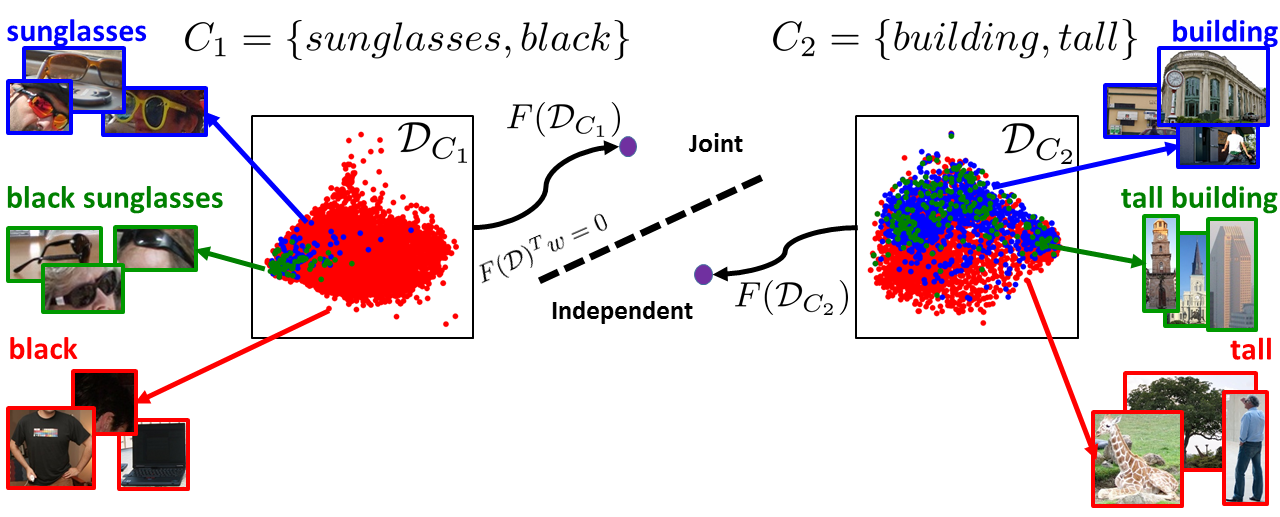
\includegraphics[width=0.8\linewidth]{teaser5.png}
\caption{{\bf Method overview:} given a visual composite $C_i$ and the corresponding training data $\mathcal{D}$ (illustrated by tSNE plot of the CNN image features), statistical features $F(\mathcal{D})$ are extracted. The resulting vectors are used to determine which training strategy should be used for each specific composite, using a trained regressor. Our method chooses to train {\em black sunglasses} as a joint phrase and {\em tall building} as an independent product of {\em tall} and {\em building} classifiers.} % Illustrated tSNE-projected distributions over samples give an insight to this selection.}
\label{fig:teaser}
\vspace{-0.1in}
\end{figure}

%-------------------------------------------------------------------------
\section{Related work}

% \cite{Rastegari2013,Gupta2009,Lan2013,Choi2010,Desai2012,Li2012,Sadeghi2011,Yao2010,Johnson2015,Chai2013,Mensink2014,Gupta2009,Farhadi2009,Farhadi2010,Lampert2013,Sadeghi2015,Felzenszwalb2010,Gupta2009,Malisiewicz2009,Chen2013,Zhu2014,Zitnick2014,Matikainen2012,Wang2015,Yao2012}

This work is related to a number of core topics in computer vision, including contextual object detection, scene understanding, scene parsing and visual language grounding. Here we review only the most relevant literature. 

\vspace{0.05in}
\noindent
{\bf Object detection:} Most object detection algorithms treat each object category independently and build independent classifiers/detectors using standard supervised learning methods (\eg, SVM, structured SVM, or latent SVM) based on hand-designed (\eg, HOG \cite{Dalal2005}) or learned features. Until recently, discriminative part-based (DPM) models \cite{Felzenszwalb2010} were particularly popular, due to their ability to compactly model appearance variations of objects while maintaining geometric relationships among parts \cite{Yang2011}. However, with recent advances in deep learning, there has been a shift to methods that either obtain a set of object proposals (\eg, obtained using selective search \cite{Uijlings2013}) and then use a CNN for classification (\eg, R-CNN \cite{Girshick2014}), or use CNN models that are trained to directly regress bounding box along with object category label \cite{Szegedy2013}. Our approach builds upon the newer R-CNN formulation \cite{girshick15fastrcnn} combined with SVM and probabilistic score re-scaling (similar to \cite{Johnson2015}) as the basic detection model. However, our main observations and conclusions are independent of the specific detection model. 

\vspace{0.05in}
\noindent
{\bf Contextual object detection:} Relatively early, in vision, it was hypothesized that contextual relationships among objects in scenes are very important for recognition. A number of works modeled co-occurrence between object categories by detecting individual objects and modeling their relative locations (and scales) using spatial distributions. Gupta \etal~\cite{Gupta2008} used prepositions and adjectives to relate nouns (objects); Hoiem \etal~used geometric relationships to reason about location and scale of objects in street scenes \cite{Hoiem2006}. For a specific class of human-object context, Yao \etal~\cite{Yao2010} proposed a joint DPM model for a person and manipulated object. Gupta \etal~\cite{Gupta2009} propose a Bayesian approach, which integrated various functional constraints and coherent semantic interpretation. 

\vspace{0.05in}
\noindent
{\bf Scene understanding:} More generic multi-object relationships were explored in \cite{Li2012}, where groups of objects that geometrically co-occurred were mined and modeled. A discriminative holistic model for scene understanding that combined segments, objects and scene labels was introduced in \cite{Yao2012}. Particularly relevant is the recent work on semantic image retrieval \cite{Johnson2015}, that introduced the concept of scene graphs -- a construct, closely related to scene parsing, design to represent objects (\eg, {\em man}, {\em boat}), attributes of objects (\eg, {\em boat is white}) and relationships between objects (\eg, {\em man standing on boat}).

However, all of these methods neglect to model the change in the appearance of an object due to interaction with another object and/or the attribute it possesses. For example, {\em person sitting} may look very different and potentially easier to detect than {\em person} and {\em sitting} that happen to co-occur in the same spatial location. In other words, above methods assume appearance independence, in order to express the object-object or object-attribute relationships using an MRF or CRF \cite{Choi2010,Johnson2015,Yao2012}. Our approach does not make this assumption, and instead tries to determine if joint appearance variation is useful and model it.

\vspace{0.05in}
\noindent
{\bf Phrases and visual composites:} In an attempt to model induced object-object appearance changes, Malisiewicz \etal~\cite{Malisiewicz2009} introduced a {\em visual memex} model that modeled visual similarity and spatial context between object exemplars using a graph. The concept of visual phrases was introduced by Sadeghi \etal~\cite{Sadeghi2011}. In \cite{Sadeghi2011} it was shown that training joint detectors for phrases (\eg, {\em man riding horse}), as opposed to individual objects (\eg, {\em man}, {\em horse}), resulted in better performance, despite fewer training instances being available to train each joint phrase classifier. This idea was further extended in \cite{Lan2013} by discovering visual composites and their spatial relations, through unsupervised sub-categorization. % , as opposed to explicit image labeling. 

One important observation is that while these methods showed that performance {\em on average} increases by jointly modeling object-object appearance, this is not the case for {\em all} object category pairs considered. 
% For example, as reported in \cite{Sadeghi2011}, in \cite{Desai2010} phrase-based recognition outperforms phrase-less recognition on $6$ out of the $8$ classes ({\em chair} and {\em horse} categories did not improve). Similarly using decoding of \cite{Sadeghi2011} on {\em  bottle} was at par with and without phrase context. This suggests that joint appearance modeling is not universly beneficial. 
Building on this intuition, in \cite{Sadeghi2015}, a model for visual knowledge extraction and visual verification of relational phrases was introduced. To verify relational predicates (\eg, {\em fish}({\em bear}, {\em salmon})), a model that considers all combinations of detectors is considered (\eg, {\em bear}, {\em salmon}, {\em bear fishing}, {\em fishing salmon} and {\em bear fishing salmon}); the scores of all of these detectors are combined using a form of CRF on a factor graph. 

Our method builds on similar intuition as \cite{Sadeghi2015}, however, instead of building all possible partial detectors and combining their scores (which is expensive and potentially sub-optimal), we attempt to choose which of the detectors for the given relational predicate 
% (\eg, of the form {\em  attribute(object)} or {\em relation(subject, object)}) 
would be most accurate and train only that specific detector. As a consequence, our model is no more expensive to evaluate and train than a model that assumes independence,
% among objects, objects and their attributes, and/or scenes and their attributes, 
yet allows us to jointly model induced appearance variations when deemed necessary. 

\vspace{0.05in}
\noindent
{\bf Attributes:}  In addition to object-object relationships we also apply our model to attribute-object and attribute-scene relationships. Attributes have received a lot of attention in vision \cite{Farhadi2009,Lampert2013} and tend to refer to namable mid-level semantic concepts 
% % (adjectives) 
related to object or scenes (\eg, person {\em sitting}, {\em man-made} scene). Our work is most closely related 
% and conceptually similar 
to \cite{Rastegari2013}, where authors propose a method for determining whether for multi-attribute queries one should train independent classifiers (one for each attribute) or conjunctions of attributes. Importantly, they identify conjunctions to train without explicitly training all combinations of classifiers. We take a conceptually similar approach but learn how to determine which ``conjunction" classifiers to train (as opposed to relaying on inter- and intra- class variances) and apply our method to a broader set of problems. %  and domains.  

% \vspace{0.05in}
% \noindent
% {\bf Model recommendation:} Model recommendation \cite{Matikainen2012,Wang2015} attempts to predict which classifier (or sets of classifiers) is best to use at test time. However, unlike our model, it requires pre-training all possible classifiers ahead of time and only does the selection at test time. Hence our proposed notion of selecting which classifier to train is much less expensive.  

%\vspace{0.05in}
%\noindent
%{\bf Statistical independence tests:} 




%-------------------------------------------------------------------------
\vspace{-0.05in}
\section{Method}

Given a visual composite (\eg, man holding a phone) we define the problem of choosing how to model and train the detector for this composite as {\em strategy selection}. We first make the empirical observation that non-uniform strategy selection can be beneficial (Section~\ref{sec:visual_phrases}). Even though one strategy is dominant on {\em average}, some composites tend to perform better when modeled and trained using one of the alternative strategies. It is therefore intuitive that a careful selection of a training strategy {\em per composite} can boost performance, regardless of the task, as shown in Table~\ref{tab:joint-ind}. With this observation in mind, we aim to predict for each composite the training strategy that will result in optimal performance (Section~\ref{sec:learning_strategy}). A reliable prediction is the performance measured on a validation set. However, pre-training all detectors for various strategies and cross-validating across them is computationally expensive.
In order to avoid pre-training, we learn a proxy function using statistical features extracted from the training samples and validation results of previously observed composites. Given a new composite, we apply this function to select its training strategy. 
% We first present the basic classification scheme used throughout the paper and then describe in detail the prediction model and statistical features it is using. 

% We first present the basic evaluation scheme to be used throughout the paper, and then describe in detail our prediction method and features being used.
\vspace{-0.2cm}
\subsection{Base model for detection}

We formulate our base model following recent state-of-the-art methods for detection and classification. However, the exact form of the model is largely independent of our main findings. In particular, we represent each image (or an image patch) $i$ using a feature vector $\mathbf{x}_i \in \mathbb{R}^{4096}$ from the last fully-connected layer (fc7) of a CNN network. We then train a detector using a linear SVM (similarly to the process described in \cite{Johnson2015}), and further calibrate the SVM scores to obtain probability estimates. 
% More formally, we solve the following problem for each class:
% \begin{eqnarray*}
% \min_{\mathbf{w}_c, b,\xi} && \frac{1}{2} \mathbf{w}_c^T \mathbf{w}_c 
% + C \sum_{i=1}^N \xi_i  \\
% \text{s.t} &&  y_i (\mathbf{w}_c^T \mathbf{x}_i + b) \geq 1 - \xi_i,  ~~~~ \forall i
% \end{eqnarray*}
% where $\mathbf{w}_c$ is the learned weight vector for class $c$ SVM classifier and $y_i$ is a binary variable which is defined to be $1$ if a given image/patch $i$ is labeled as class $c$ and $-1$ if it is not. 
The calibration is implemented using Platt scaling \cite{Platt99probabilisticoutputs}:
\begin{eqnarray*}
P(y_c=1|\mathbf{x}_i)=\frac{1}{1+e^{\alpha_c(\mathbf{w}_c^T \mathbf{x}_i + b) +\beta_c}},
\end{eqnarray*}
% \RevComment{I’d suggest dropping a few of the equations - they’re well-known- svm, ridge regression), and take up a ton of space. In terms of selling the paper too, they give a clear tip-off that this isn’t an end-to-end trained CNN paper. Personally, I’m not bothered by that, but I wouldn’t advertise it given the frequency of angsty grad student reviewers.}
where $\alpha_c,\beta_c$ are the calibration coefficients; $\mathbf{w}_c$ and $b_c$ are the learned SVM weights and bias, respectively, for class $c$.

For object detection, we use labeled bounding boxes containing objects as positive samples and use CNN adapted for detection tasks \cite{girshick15fastrcnn} to compute $\mathbf{x}_i$. For scene classification, we use labeled full images and a neural network fine-tuned for scene classification \cite{NIPS2014_5349} to define our positive samples. In both cases, negative patches/images are extracted from the training data. For detection, we perform multiple rounds of retraining using hard negative mining for further learning refinement. When applying object detector, at test time, we use an object proposal scheme \cite{Uijlings2013} to generate plausible hypotheses. 

Note that if we want to build a detector for a relatively complex visual composite entity, \eg, $C = man~sitting$, we can do this using one of two ways: (1) assuming {\em independence}, i.e., 
$P(y_{C} = 1 | \mathbf{x} ) = P(y_{man} = 1 | \mathbf{x}) P(y_{sit} = 1 | \mathbf{x})$, or (2) by building a {\em joint} detector for the full visual phrase -- $P(y_{man~sitting} = 1 | \mathbf{x} )$. Detectors involved in (1) have the benefit of being trained from a larger set of samples, but may need to capture wider visual variances. Detector (2) has the benefit of modeling a presumably narrower visual variance, but could potentially lack sufficient number of samples to train a good model. As such, we posit that the performance of the two will be different at runtime, in general, and one will likely perform better than the other under certain conditions (see Table~\ref{tab:joint-ind}). Before studying the benefits of these strategies, we first more formally define the visual composite constructions that we use in the remainder of the paper. 




% Given an image, we use CNNs for feature extraction. For object detection tasks we use \cite{Uijlings2013} to generate object proposals for each image, and represent each proposal as the vector extracted from the last fully-connected layer (fc7) of a neural net adapted for detection tasks \cite{girshick15fastrcnn}. For scene recognition, we propagate each image through a a neural network fine-tuned for similar tasks \cite{NIPS2014_5349} to obtain its fc7 representation. We then train each class detector using a linear SVM(similarly to the training process described in \cite{Johnson2015}), and further calibrate it to obtain probability estimates. More foramally, we solve the following problem for each class:\Guy{decide how deep we dive into the details here}
% \begin{eqnarray*}
% x_i=\Phi_{NN}(I)\\
% y_i=
% \begin{cases}
%     1 & \text{if } I \in \{C\}\\
%     0,              & \text{otherwise}\\
% \end{cases} \\
% \min_{w_c,b,\xi} && \frac{1}{2} w_c^T w_c 
% + C \sum_{i=1}^N \xi_i  \\
% \text{s.t} && y_i (w_c^T x_i + b) \geq 1 - \xi_i 
% \end{eqnarray*}
% Note that joint categories are trained with the subset of positive examples annotated with all composite parts. These trained detectors are in turn applied on test images for evaluation: given a single composite as a query, we perform 2 processes - independent and joint. we once apply all independent detectors included in the composite and multiply their scores. In parallel, we apply the joint composite detector. Thus we have 2 different estimates for each object proposal or images, that can be evaluated in various methods. For example, given the composite \{man is sitting\} in an object detection task, for each object proposal $b$ we have $P_i(b)=P(man)P(sitting)$,$P_j(b)=P(man,sitting)$, where $P_i,P_j$ are the independent and joint estimates, correspondingly.   

%Each image in the dataset is annotated with a single scene (\eg, baseball field), and possibly multiple attributes (\eg, outdoor). We use a neural network fine-tuned for similar tasks \cite{NIPS2014_5349} to represent each image as an output of the last fully connected layer. Again, we train a linear SVM for each category and calibrate scores. For evaluation we use a single scene+attribute as a query, rank the test images according to the scores obtained from the corresponding classifiers and compute mean average precision.
%We perform the following experiment:
%\begin{itemize}
%\item {{\bf\{att,scene\}}: a single joint strategy, train \{att+scene\} category. The independent strategy is the same as in \{obj,att\}.}
%\end{itemize}

%\subsection{Motivation}
%It is quite clear that some visual composites are optimally learned as a whole, while others should be addressed by learning a function for each composite part. Assuming that a given dataset is not heavily biased towards one strategy, one can boost performance quality by an optimal strategy selection. For the datasets described in this paper, we gain an average of \% x \Guy{compute} in performance by such optimal selection. Obviously, this selection is latent and can only be approximated. An exhaustive approach would involve pre-training a composite using all available strategies, and make a selection according to performance on validation set. Despite being a good approximation, it is computationally expensive. Therefore, predicting the optimal selection without actually using training is highly desirable. Our method can achieve comparable results to a cross-validation approximation, with a fraction of the computational cost. 
\vspace{-0.2cm}
\subsection{Visual composites}
\label{sec:visual_phrases}
% \RevComment{Overall the paper is consistent with notation, but some issues in notation remain, and an extra pass over notation would probably help iron them out. I would try and look for opportunities to minimize the amount of notation in Section 3.2, although I do not have concrete suggestions for how to do so.}
Consider a visual composite $C \in \mathcal{C}$ consisting of $N$ parts (or word tokens), \ie, $C = \{ c_1, c_2, ...,  c_N \}$, where each part/word token, $c_i \in \{\mathcal{O}, \mathcal{A}, \mathcal{R} \}$, can be a noun from a predefined set of noun object (or scene) categories $\mathcal{O}$ (\eg, ``man", ``horse"), an adjective from a set of visual attributes describing objects (or scenes) $\mathcal{A}$ (\eg, ``tall", ``bold", ``open"), preposition and/or verb from a set of predefined object relationships $\mathcal{R}$ (\eg, ``in", ``next to", ``holding", ``riding"}). 

For example, in the composite $C=${\em ``man holding phone''},  $\{c_1 = o_1 =``man" \in \mathcal{O}, c_2 = r = ``holding" \in \mathcal{R}, c_3 = o_2 = ``phone" \in \mathcal{O} \}$. In general, if we want to detect or ground $C$, given an image $\mathbf{x}$, we have a number of options available to us, as alluded to in the previous section. Specifically, if we treat each part/token {\em independently}, we obtain the traditional formulation \cite{Johnson2015}:
%
\begin{eqnarray}
\mathbf{b}^{*}_{1},\mathbf{b}^{*}_{2} & = & \operatornamewithlimits{argmax}_{\mathbf{b}_1,\mathbf{b}_2} P(y_{C}=1 | \mathbf x) \nonumber \\
& = & 
\operatornamewithlimits{argmax}_{\mathbf{b}_1,\mathbf{b}_2} P(y_{o_1}=1|\mathbf x_{\mathbf{b}_1})P(y_{o_2}=1|\mathbf x_{\mathbf{b}_2})P(\mathbf{b}_1,\mathbf{b}_2|r),
\label{eq:indep}
\end{eqnarray}
%
\noindent
where $\mathbf{b}_1$ and $\mathbf{b}_2$ are the bounding boxes for $o_1$ and $o_2$, respectively,
$\mathbf{x}_{\mathbf{b}_1}$ and $\mathbf{x}_{\mathbf{b}_2}$ are corresponding CNN features of the image patches enclosed by these bounding boxes and $P(\mathbf{b}_1, \mathbf{b}_2|r)$ is a spatial distribution for relationship $r$ (\eg, a Gaussian mixture model \cite{Johnson2015}), designed to encode spatial consistency between two object patches. Alternatively, the problem can also be expressed in the following ways:
%
\begin{eqnarray}
\mathbf{b}^{*}_{1},\mathbf{b}^{*}_{2} 
& = & 
\operatornamewithlimits{argmax}_{\mathbf{b}_1,\mathbf{b}_2} P(y_{o_1}=1|\mathbf x_{\mathbf{b}_1})P(y_{o_2+r}=1|\mathbf x_{\mathbf{b}_2})P(\mathbf{b}_1,\mathbf{b}_2|r), \label{eq:joint_o2r} \\
& = & 
\operatornamewithlimits{argmax}_{\mathbf{b}_1,\mathbf{b}_2} P(y_{o_1+r}=1|\mathbf x_{\mathbf{b}_1})P(y_{o_2}=1|\mathbf x_{\mathbf{b}_2})P(\mathbf{b}_1,\mathbf{b}_2|r), \label{eq:joint_o1r}\\
& = & 
\operatornamewithlimits{argmax}_{\mathbf{b}_1,\mathbf{b}_2} P(y_{o_1+r}=1|\mathbf x_{\mathbf{b}_1})P(y_{o_2+r}=1|\mathbf x_{\mathbf{b}_2})P(\mathbf{b}_1,\mathbf{b}_2|r), \label{eq:joint_o1o2r}\\
& = & 
\operatornamewithlimits{argmax}_{\mathbf{b}_1,\mathbf{b}_2} P(y_{o_1+r+o_2}=1|\mathbf x_{\mathbf{b}_1 \cup \mathbf{b}_2}), \label{eq:full_joint}
\end{eqnarray}
%
where, for example, $P(y_{o_1+r}=1|\mathbf x_{\mathbf{b}_1})$ and $P(y_{o_2+r}=1|\mathbf x_{\mathbf{b}_2})$ are classifiers trained to detect {\em ``man holding"} and {\em ``holding phone"} phrases respectively. The difference in these formulation is assuming less appearance independence from top to bottom. Note that for a general visual composite of length $N$, the number of ways to model the classifier becomes exponential.
%: $2^{(N-1)}+1$.\RevComment{I don’t follow how to arrive at the $2^{N-1} + 1$ number, though I agree it’s exponential in the number of labels. Also, it would be useful to use a letter/symbol other than N, which seems to be used for the number of training images in the next paragraph.} 

Our overall goal is to determine which of the Eq. (\ref{eq:indep})--(\ref{eq:full_joint}), that determines the learning strategy, would result in the most accurate model at testing time. Even more fundamentally, if the choice of a strategy matters and when? 
%
In this work, we make a simplifying assumption that we only look at joint vs. independent modeling of simple noun phrases, mainly object-attribute or object-relationship phrases. Therefore, we effectively restrict ourselves to a choice among Eq.(\ref{eq:indep})--(\ref{eq:joint_o1o2r}) for strategy selection on $C$. % Note that for the special case of scene-attribute we let $\mathbf{b}_1$ and $\mathbf{b}_2$ be full images, do away with relationships and term $G$ and use $a \in \mathcal{A}$ instead of $r \in \mathcal{R}$ within equations above.  

To train the corresponding classifiers, we assume that we are working in a fully supervised setting with an annotated dataset of $N$ training images, $\mathcal{D}_{\mathcal{OA}} =\{ ( \mathbf{b}_{i,j}, \mathbf{l}_{i,j} ) \}$, where $i \in [1, N]$ is the image index and $j \in [1, B_i]$ is defined over a set of $B_i$ annotated regions in $i$. The variable $\mathbf{b}_{i,j} \in \mathbb{R}^4$ then denotes the bounding box of the corresponding image region and $\mathbf{l}_{i,j} = ( o_{i,j}, \mathbf{a}_{i,j} )$ denotes the set of assigned labels, where $o_{i,j} \in \mathcal{O}$ is an object label and $\mathbf{a}_{i,j} = \{ a_{i,j,k} \}$ is a potentially empty set of attributes $a_{i,j,k} \in \mathcal{A}$ taken from an attribute set $\mathcal{A}$, where $K_{i,j}$ is the total number of attributes assigned to region $j$ in image $i$ and $k \in [1, K_{i,j}]$. For example, for a region $j$ in image $i$ labeled ``tall old person", $K_{i,j} = 2$ and $\mathbf{l}_{i,j} = (person, \{ tall, old \} )$. In addition, each pair of bounding box annotations in a given image $i$ can be associated with a set of relationship, such that $\mathcal{D}_{\mathcal{R}} = \{ (\mathbf{b}_{i,j}, \mathbf{b}_{i,k}, \mathbf{r}_{i,j,k} ) \}$. For example, annotation ``person holding and swinging the racket", would correspond to $\mathbf{r}_{i,j,k} = \{ holding, swinging \}$. Further, with slight abuse of notation we define data subsets: 
\vspace{-0.05in}
\begin{eqnarray}
\mathcal{D}_{\mathcal{O} = \hat{o}} & = & \{ ( \mathbf{b}_{i,j}, \mathbf{l}_{i,j} ) | \forall i, \forall j ~\text{s.t.}~ o_{i,j} = \hat{o}  \},\nonumber \\
\mathcal{D}_{\mathcal{A} =  \hat{a}}} & = & \{ ( \mathbf{b}_{i,j}, \mathbf{l}_{i,j} ) | \forall i, \forall j, \exists k ~\text{s.t.}~ a_{i,j,k} = \hat{a} \}, \nonumber \\
\mathcal{D}_{\mathcal{R} = \hat{r}} & = & \{( \mathbf{b}_{i,j}, \mathbf{b}_{i,k}, \mathbf{r}_{i,j,k}) | \forall i, \forall j, \exists k~\test{s.t.}~\mathbf{r}_{i,j,k} = \hat{r} \}, \nonumber \\
\mathcal{D}_{\mathcal{O} = \hat{o}, \mathcal{A} = \hat{a}} &  = & \mathcal{D}_{\mathcal{O} = \hat{o}} \cap \mathcal{D}_{\mathcal{A} = \hat{a}}; ~~
\mathcal{D}_{\mathcal{O} = \hat{o}, \mathcal{R} = \hat{r}}  =  \mathcal{D}_{\mathcal{O} = \hat{o}} \cap \mathcal{D}_{\mathcal{R} = \hat{r}}. \nonumber
\end{eqnarray}
We note that for scene-attribute scenario, the setting is somewhat simplified by effectively setting $\mathbf{b}_{i,j}$ to full images, and not having $\mathcal{D}_{\mathcal{R}}$.
% and hence also $\mathcal{D}_{\mathcal{R}=\hat{r}}$ or $\mathcal{D}_{\mathcal{O} = \hat{O}, \mathcal{R} = \hat{r}}$.
Overall, we consider the following choices of joint vs. independent selections:
%
%
% Consider a visual composite $C$ consisting of $N$ parts (or word tokens), \ie, $C = \{ c_1, c_2, ...,  c_N \}$, where each part $c_i \in \{\mathcal{O}, \mathcal{A}, \mathcal{R} \}$ with $\mathcal{O}$ be a set of object (or scene categories) categories, $\mathcal{A}$ a set of visual attributes or adjectives describing objects (or scenes) and optional $\mathcal{R}$ which corresponds to object relationships consisting of prepositions and/or verbs. For example, in the composite $C=${\em ``man riding horse''},  $\{c_1,c_2,c_3\} = \{man \in \mathcal{O}, riding \in \mathcal{R}, horse \in \mathcal{O} \}$. In general, if we want to detect $C$, \ie, build a probailistic classifier $p(y_C=1|\mathbf{x})$ given an image patch $\mathbf{x}$, we have a number of options as alluded to in the previous section. Specifically, in addition to treating each part independently, we can  
%
% Given a visual composite, it can be disassembled to its parts. Let us denote a composite as $C \triangleq$ $\{c_1,c_2,..,c_N,D\}$, when $c_i$ is a composite part, and $D$ is training subsets of composite parts: $D \triangleq$ $\{d_{c_1},d_{c_2},..,d_{c_N}\}$, when $d_{c_i}$ is the subset of data containing all training examples for $c_i$. For example, in the composite {\em ``man riding horse''},  $\{c_1,c_2,c_3\}$ = \{man,riding,horse\} and $D=\{d_{man},d_{ride},d_{horse}\}$. Note that for different parts $i\neq j$, $d_i$ and $d_j$ can still have overlapping training examples. To train an {\em independent} composite detector, we train $P(y_{c_i}=1|\mathbf x)$, where \mathbf x is sampled from $d_{c_i}$. To train a {\em joint} detector for 2 composite parts, we train $P(y_{c_i,c_j}=1|\mathbf x)$, where \mathbf x is sampled from $d_{c_i} \cap d_{c_j}$. Specifically, we focus on the following {\em composite} types:
%
\vspace{-0.05in}
\begin{itemize}
\item {\bf scene-attribute}: we choose between $P(y_{s}=1|\mathbf{x})$
$P(y_{a}=1|\mathbf{x})$ and 
$P(y_{s+a}=1|\mathbf{x})$ trained with 
$\mathcal{D}_{\mathcal{O}=s}$, $\mathcal{D}_{\mathcal{A}=a}$
and $\mathcal{D}_{\mathcal{O}=s, \mathcal{A}=a}$ respectively.
\vspace{0.05in}
\item {\bf object-attribute}: we choose between $P(y_{o}=1|\mathbf{x}_{\mathbf{b}})$
$P(y_{a}=1|\mathbf{x}_{\mathbf{b}})$ and 
$P(y_{o+a}=1|\mathbf{x}_{\mathbf{b}})$ trained with 
$\mathcal{D}_{\mathcal{O}=o}$, $\mathcal{D}_{\mathcal{A}=a}$
and $\mathcal{D}_{\mathcal{O}=o, \mathcal{A}=a}$ respectively.
\vspace{0.05in}
\item {\bf object-relationship-object}: where we choose among the choices denoted in Eq.(\ref{eq:indep})--(\ref{eq:joint_o1o2r}) trained with respective data subsets. 
\end{itemize}
\vspace{-0.05in}

% such composite has a single joint strategy, training joint object+attribute category. In such case we measure the mean IoU on test images containing bounding boxes annotated with both object and attribute. 

% {\bf object,relationship,object}: such composite  contains multiple joint strategies: 
% \begin{enumerate}
%     \item obj$_1$+rel,obj$_2$
%     \item obj$_1$,rel+obj$_2$
%     \item obj$_1$+rel,rel+obj$_2$
% \end{enumerate}
% For example, for {\em man,riding,horse} we can use the 2 independent man,horse detectors, or use one of the following joint detectors:[man+riding,horse], [man,riding+horse], [man+riding,riding+horse]. We use scores of the 2 detectors and select our object proposals according to the following product:
% \begin{equation}
% b^{*}_{1},b^{*}_{2}=\operatornamewithlimits{argmax}_{b_1,b_2} P(y_{c_1}=1|\mathbf x_{b_1})P(y_{c_2}=1|\mathbf x_{b_2})G(b_1,b_2|rel)
% \end{equation}
% Where $G(b_1,b_2|rel)$ is a Gaussian mixture model trained for each relationship, following the formulation in \cite{Johnson2015}. In such case we average the IoU of the object pair for evaluation.

% {\bf attribute,scene}: such composite contains a single joint strategy, training attribute+scene category. At run time we measure mean average precision for each joint class for evaluation.

Table~\ref{tab:joint-ind} (left two rows) illustrate example performance results of the {\em independent} and the various {\em joint} strategy(ies) for individual object-attribute and object-relationship-object\footnote{For object-relationship-object joint strategy we report the best perfromance among $3$ joint strategies considered.} composites. One key observation is that for certain composites one strategy performs significantly better than the other.
%, \eg, for ``street-black" the performance of the {\em jointly} trained detector, in terms of IoU of the bounding boxes across the test set, is 62\% better than the {\em independently} trained detector. 
Further, notice that both {\em independent} and {\em joint} training strategies are useful. In particular note that the optimal stategy is not necessarily the function of the object, but rather of the composite as a whole (\eg, for ``street-black" joint detector is better, where as for ``street-paved" independent detector leads to 22\% improvement). This raises the issue of how one should select the best strategy in each case, which we will address in the next section.  


%\Guy{Added table.not sure how to represent validation - binary desicion/diff in performance?}

\begin{table}[t]
\begin{center}
 \begin{tabular}{|c || c | c | c | c | c ||} 
 \hline
  & \multicolumn{2}{|c|}{Performance} & \multicolumn{3}{|c||}{Prediction}  \\ \hline
  Composite Phrase & Independent & ~~~Joint~~~  & Validation & Our Model & Improvement\\ [0.5ex]
 \hline\hline
 laptop-white & 0.353 & \textbf{0.409} & +0.173 & -0.064 & -15.8\%\\ 
 \hline
 street-black & 0.375 & \textbf{0.608} & +0.133 & +0.005 & +62.1\%\\
 \hline
 street-paved & \textbf{0.594} & 0.486 & -0.091 & -0.092 & +22.2\%\\
 \hline
 hair-black & 0.209 & \textbf{0.234} & +0.030 & +0.022 & +11.9\%\\
 \hline
 tracks-metal & 0.383 & \textbf{0.414} & +0.054 & +0.001 & +8.1\%\\
 \hline
 bench-wood & \textbf{0.298} & 0.196 & -0.087 & -0.025 & +52.0\%\\ 
 \hline
 % man-riding-horse & \textbf{0.500} & 0.378 & -0.066 & -0.038 & +32.2\%\\
 \hline
 man-holding-phone & 0.241 & \textbf{0.265} & +0.011 & +0.018 & +9.9\%\\
 \hline
 man-behind-man & 0.203 & \textbf{0.230} & +0.047 & -0.032 & -13.3\%\\
 \hline
 woman-next to-bus & \textbf{0.439} & 0.328 & -0.046 &  -0.022 & +14.0\%\\
 \hline
\end{tabular}
\end{center}
\caption{Some examples of the actual performance of the two strategies, joint or independent, for detectors on various visual phrases in SceneGraph dataset. Note that there is no clear strategy that outperforms the other on all phrases. On the left we show the cross validation prediction and our method's prediction for the difference in performance.}
\label{tab:joint-ind}
\vspace*{-\baselineskip}
\vspace*{-\baselineskip}
\end{table}

\vspace{-0.05in}
\subsection{Predicting Learning Strategy}
\label{sec:learning_strategy}

As no single strategy for training detectors is better for all cases, there is a need to choose the optimal strategy for each composite phrase. One possibility for determining this is to use a subset of the data for \emph{cross validation}. In this case all types of detectors are tested on the cross validation data and the best strategy is chosen as the detector. Table~\ref{tab:joint-ind} shows the results of the cross validation strategy in (Validation) column, where ``+" designates preference of the cross validation for the {\em joint} strategy and ``-" designates preference for the independent strategy (the value itself predicts the strength of the preference, which corresponds to the maximum absolute difference between the cross validation performance of the independent and the best joint strategy). 
Using cross-validation, however, may be extremely time consuming and error prone. Specifically, for the case of object-relationship-object phrases we need to train $4$ separate classifiers and evaluate them on a validation set to choose an appropriate strategy. If we start to consider longer composites or multi-class classification/detection strategies, the space of possible strategies starts to grow exponentially and cross validation becomes much more expensive. Further, from a practical point of view, in many cases there may not be enough data for cross validation which may result in high variance in strategy selection. To address these issues, we propose a method for learning how to choose an optimal strategy without explicitly training all the detectors. To this end, we propose a simple regression scheme defined on a set of features extracted from the training sample sets.

\vspace{0.1in}
\noindent
{\bf Regression:}
Our key idea is simple but surprisingly effective. We use cross validation on $\mathcal{C}_{tr}$ - a small fraction of composites (20\%-30\%), to learn to predict the preference between the two strategies. We do this by first training and measuring cross-validation performance for this small subset of composites. We then use a set of features of the corresponding training samples to regress the difference in cross-validation performance (the values in the (Validation) column of the Table~\ref{tab:joint-ind}). The learned regressor can then serve as a predictor on new composites to choose which strategy to use for the remainder of the composites. 

Let $S = \{ I, J_1, J_2, .., J_M\}$ denote the set of $M+1$  possible training strategies\footnote{For example, all object-attribute pairs would share the same set of strategies.}, where $I$ and $\{J_{m}\}\limits_{m=1}^M$ are the independent and (possibly multiple) joint strategies, respectively. 
Let $P_s(y_C | \mathbf{x})$ be the resulting trained classifier for composite $C$ with strategy $s$.  
By applying $P_s(y_C | \mathbf{x})$ on a validation set we can obtain validation accuracy, which we denote $V_{s,C}$. Our goal is to train a regressor to predict $V_{s,C}$ from the features of the data sub-set, lets call it $\mathcal{D}_C$, used for training $P_s(y_C | \mathbf{x})$ directly. For this we define a feature mapping $\mathbf{f}_C = F(\mathcal{D}_C)$, discussed in detail in the next section. 
In practice, we actually predict the differences $V_{J_m,C} - V_{I,C}$, instead of each $V_{s,C}$, learning a linear prediction models as follows:
%A validation accuracy evaluation metric is denoted as $V(\cdot)$, and a feature extraction operator by $F(\cdot)$. We are given a group of previously observed composites, along with their validation set performances for each strategy: $\{V(t_{I,c}),V(t_{J_{1},c}),...,V(t_{J_{K},c}))\}\limits_{c=1}^{|\mathcal{C}|}$. For each joint strategy $J_m$ we learn a linear regressor, using features extracted from the training samples $\mathcal{D}$ for each sub-set used to train $t_{I,c}$. More specifically, we solve the following optimization problem:
%
\vspace{-0.3cm}
\begin{align}\label{first}
\mathbf{w}_m = \operatornamewithlimits{argmin}_{\mathbf{w}}\sum\limits_{C=1}^{|\mathcal{C}_{tr}|} (\mathbf{f}_{C}^{T} \mathbf{w} - [V_{J_m,C} - V_{I,C}])^2 + \lambda|| \mathbf{w}||_2^2,
\end{align}
%
where the second term is is a regularizer with a weight $\lambda$ (we experimentally set $\lambda = 0.01$). Simply put, we are regressing the difference in performance between an independent and each available joint strategy, measured on a validation set. 

Given the learned regression, when observing a new composite $C_{new}$, our model makes a selection of the strategy, $s_{new} \in S$ according to the following prediction rule, which no longer requires training of different strategies for $C_{new}$ or evaluation of resulting classifiers on validation data:
%
\begin{equation}
\begin{align}
% m^* = \operatornamewithlimits{argmax}_{m} \mathbf{f}_{C_{new}}^{T}\mathbf{w}_m \\
s_{new}= 
\begin{cases}
    J_{m^*}& \text{if } \mathbf{f}_{C_{new}}^{T} \mathbf{w}_{m^{*}} > 0\\
    I,              & \text{otherwise}
\end{cases}
\text{, where~~} 
m^* = \operatornamewithlimits{argmax}_{m} \mathbf{f}_{C_{new}}^{T}\mathbf{w}_m.
\end{align}
\end{equation}
%
The above formulation predicts {\em independent} strategy ($I$) when it is predicted to outperform all {\em joint} strategies, otherwise, joint strategy with largest predicted margin of improvement ($J_m^*$) is returned. Now we turn our attention to formalizing the features $\mathbf{f}_C$ used in above prediction model.

%Note that we are coupling strategy pairs when obtaining our regression targets, as we are aiming to learn the relative gain for a given strategy, rather than learning a single strategy independently.

\vspace{0.1in}
\noindent
{\bf Feature extraction:}
We hypothesise that the {\em topology} of training examples for a given composite contains informative cues for the strategy selection. Our feature selection rises from the intuition that it should capture the trade-off between cardinality and compactness of the samples, as suggested by \cite{Rastegari2013}. Recall that $\mathcal{D}_c$ is the data subset for a single composite part. We use $\mathcal{D}_c$ to extract a feature vector $\mathbf{f}_c = [f_{c,1}, f_{c,2}, ..., f_{c,6}] \in \mathbb{R}^{6}$ comprising:
\begin{itemize}
\item Number of samples: $f_{c,1} = |\mathcal{D}_c|$
\item Compactness of samples, represented as statistics extracted from pairwise distances:
% \begin{eqnarray*}
$\mathbf r=\{|\mathbf x_i-\mathbf x_j|\},i \neq j,\mathbf x \in \mathcal{D}_c$ encoded by 
%\end{eqnarray*}
$f_{c,2}=max(\mathbf r), f_{c,3}=min(\mathbf r), f_{c,4}=med(\mathbf r), f_{c,5}=mean(\mathbf r)$. 
We use cosine distance for $\mathbf{r}$. 
% We use cosine distance as pairwise distance metric to compute $\mathbf{r}$. 
\item Sample entropy, estimated using Nearest neighbour distance approximation:
$f_{c,6}=\frac{1}{N}\sum\limits_{i=1}^N ln(N\rho_i) + ln2 + \gamma$, where $\rho_i = min_{j\neq i} |\mathbf x_i-\mathbf x_j|$; $\gamma$ is Euler const. 
\end{itemize}

We repeat this process for each of the parts and corresponding pairwise composites and concatenate the resulting features to obtain a unified feature. For example, for $C=\{white,boat\}$ we have $F(\mathcal{D}_C) = [\mathbf f_{boat},\mathbf f_{white},\mathbf f_{white+boat}]$. 
% Although simplistic, the above feature selection empirically proves to be effective, and has a negligible computational cost in comparison to pre-training.

The last column of Table~\ref{tab:joint-ind} shows the predictions made by the learned regressor. Note, that the regressor was trained on composites other than the ones listed in the table, so it has not seen these composites during training. Even so, the regressor is able to predict the sign (which corresponds to the preference of the strategy) in $7$ out of the $9$ cases and in the two cases where it didn't, the difference between the two strategies was relatively small. 

%-----------------------------------------------------------------------
\vspace{-0.05in}
\section{Experiments}
%
% \RevComment{The gain is very small, which is fine, but the paper needs to be defensively written. I think you need one nice example (preferably some sort of subset of the data) that will shut up a reviewer who complains about this.}
%
\vspace{-0.05in}
\noindent
{\bf Datasets:} We evaluate our method for variety of detection and classification tasks. We use two public datasets. For detection and grounding, we use SceneGraph dataset  \cite{Johnson2015}; for scene classification, we use the SUN dataset \cite{patterson2014sun}. 


{\em SceneGraph dataset}~\cite{Johnson2015}
consists of $5,000$ images containing large number of object, attribute and relationship annotations (see \cite{Johnson2015} for statistics).
% over $93,000$ annotated object instances of $6,745$ object classes; $110,000$ annotated attribute instances of $3,743$ attribute classes; and $112,000$ instancees of relationships from $1,310$ relationship types. 
We use $4,000$ images for training and $1,000$ for testing using the split prescribed in \cite{Johnson2015}. We test our model in object localization task on object-attribute, object-attribute-relationship and object-relationship-object composite queries as defined in Section 6.3 of \cite{Johnson2015}. To quantitatively compare performance we report both median and mean Intersection over Union (med IoU and mean IoU) as well as the fraction of instances with IoU above various thresholds (IoU@t). 

{\em SUN dataset}: We use SUN Attribute dataset~\cite{patterson2014sun} comprising $14,340$ images from $707$ scene categories and annotated with $102$ discriminative attributes. In addition, to get more samples for each scene category, we augment each scene class in SUN Attribute with up to additional $80$ images from the full SUN dataset (less if $80$ is unavailable). 
We test our model in the context of scene-attribute retrieval task, where given a scene-attribute classifier we rank all test images in terms of their relevance to this query. We report performance using Mean Average Precision (mAP) computed on $100$ top-ranked images. We use $5$ images from each scene-attribute composite pair for testing and the rest for training. 


\vspace{0.1in}
\noindent
{\bf Baselines:} 
We implemented a number of baseline selection strategies in order to illustrate the benefits of our regression-based selection approach:

\vspace{-0.05in}
\begin{itemize}
\item {\em Optimal}: An oracle selection strategy that results in the highest performance at run-time. This is an upper bound on possible improvement in performance that can be achieved by individually choosing best strategy per composite.
\vspace{0.05in}
\item {\em Cross-validation}: Selection that consists of pre-training all strategies per composite, then selecting one that scores best on the validation set.
\vspace{0.05in}
\item {\em Independent}: Using an independent detector strategy for each and every composite. For object localization this is equivalent to model in \cite{Johnson2015}. 
\vspace{0.05in}
\item {\em Joint}: Using a joint phrase \cite{Sadeghi2011} detector for each and every composite. 
\end{itemize}
\vspace{-0.05in}

Where appropriate, we also use additional baselines consisting of threshold selection strategy on the number of joint samples and strategy proposed in \cite{Rastegari2013}.

\vspace{0.1in}
\noindent
{\bf Implementation and setup:} 
For all baselines we use the same image features, form of the detector, and the training procedure as we do for our regression-based method. We evaluate our method using 3-fold cross-validation, where regressor is trained on 30\% of composites then evaluated on the rest; reported results are averaged across the 3-folds.
% In order to evaluate our method for all available composites, we train our regressor in a holdout manner, thus predicting for each composite using a model that wasn't trained with its feature vector. All reported results are using regressors learned on 30\% of the training data, hence requiring evaluation for remaining 70\%. 
We further verify result consistency by repeating the experiments multiple times and averaging. Since it doesn't make sense to train a joint detector with very few samples, we prune composites with less training examples than a certain threshold. We plot performance as a function of this threshold (otherwise we use all composites with more than 3 joint examples). 

\vspace{-0.05in}
\subsection{Detection and Retrieval on SceneGraphs dataset}
%
% \RevComment{Table 1 is one way to view the predictions from your linear regressor, but it would be useful to also have some statistics like MSE or even just classification (use joint vs use independent) accuracy for the regressor}
%
\noindent
{\bf Object-Attribute Detection:}
We extract a total of $2,295$ ($|\mathcal{C}| = 2,295$) object-attribute composites, most frequently appearing in the SceneGraphs data-set~\cite{Johnson2015}. For evaluation we consider only joint annotations, \ie, using the subset $\mathcal{D}_{\mathcal{O} = o, \mathcal{A}= a}$ from the test set, such that combining $\{o,a\}$ results a valid composite.
% For regression, we extract features $F(\mathcal{D}) = [\mathbf f_{obj},\mathbf f_{att},\mathbf f_{obj+att}]$ for each composite.
After choosing a joint/independent strategy for each composite, we train a classifier accordingly. 
The detector works by first computing a set of object bounding box proposals, using \cite{Uijlings2013}, and then evaluating the probability of each proposal containing an object-attribute pair using the trained classifier. 
We report Average IoU computed from the top $5$ most confident detections in Figure~\ref{att_rel_perf_0.3} (left).

From Figure~\ref{att_rel_perf_0.3}, we can see that when there are many composites with low number of samples, the independent strategy performs better on average. This trend changes as the number of joint samples increases from left to right. Note that the potential gain from selecting the correct strategy is significant, as shown by the optimal curve. Learning from $0.3$ of the data, we reach performance of cross-validation at a fraction of computational cost. Using a bigger portion of data for training does not lead to significant improvement (see %Figure~\ref{fig:example} (right))
Supplementary Material). While average improvement may appear small, we do get large improvements for certain individual composites. For example, in Table~\ref{tab:joint-ind} we show that improvement for ``street-black" is 62.1\%; for ``bench-wood" 52\%. 
We can see a degradation in performance as we focus on composites with larger number of samples, due to the decrease in the number of training phrases, which results in overfitting. However, the performance with low or zero threshold (the leftmost side of the curve) is most meaningful in the realistic setting. 


%
\begin{figure}[t]
    \centering
    \subfloat{{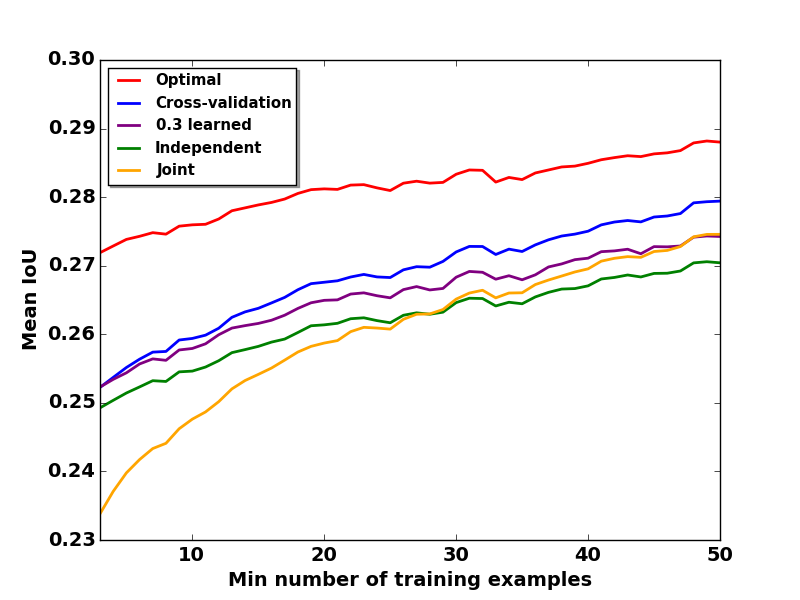
\includegraphics[width=5cm]{object_attribute_learn_partition_0_3.png} }}%
    \qquad
    \subfloat{{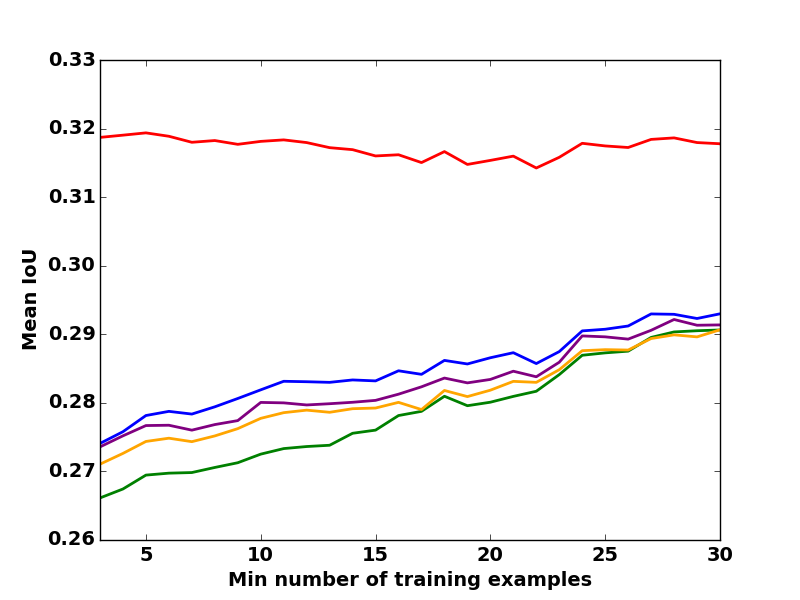
\includegraphics[width=5cm]{object_relationship_learn_partition_0_3.png} }}%
    \vspace{-0.05in}
    \caption{{\bf Detection Performance}: for composite Object-Attributes (left) and Object-Relationship-Object (right). Performance is measured in Mean IoU. Our regression-based selection method learned from 30\% of composites is denoted by ``0.3 learned". Performance is reported as a function of threshold used to filter out composites with fewer samples than the threshold shown along the x-axis.}%
    \label{att_rel_perf_0.3}
\vspace*{-0.7\baselineskip}  
\end{figure}
%

\vspace{0.1in}
\noindent
{\bf Object-Relationship-Object Detection:}
We consider $4,030$ ($|\mathcal{C}| = 4,030$) composites $C = \{o_1,r,o_2\}$ appearing both in train and test set. This results in $303$ $\{o_1+r\}$ pairs (\eg, man-holding) and $317$ $\{r+o_2\}$ pairs(\eg, holding-phone). 
% We avoid modeling a full tuple dependence due to scarce training examples.
% Eq.(\ref{eq:indep})Eq.(\ref{eq:joint_o2r})--(\ref{eq:joint_o1o2r})
In addition to an independent strategy in Eq.(\ref{eq:indep}), we consider 3 joint strategies, listed in Eq.(\ref{eq:joint_o2r})--(\ref{eq:joint_o1o2r}), thus training 3 different regressors.
% : 
% \begin{itemize}
%     \item for $P(y_{o_1+r}=1|\mathbf x_{\mathbf{b}_1}),P(y_{o_2}=1|\mathbf x_{\mathbf{b}_2}), F(\mathcal{D}) = [\mathbf f_{o_1},\mathbf f_{o_1+r},\mathbf f_{o_2}]$
%    \item for $P(y_{o_1}=1|\mathbf x_{\mathbf{b}_1}),P(y_{r+o_2}=1|\mathbf x_{\mathbf{b}_2}), F(\mathcal{D}) = [\mathbf f_{o_1},\mathbf f_{r+o_2},\mathbf f_{o_2}]$
%    \item for $P(y_{o_1+r}=1|\mathbf x_{\mathbf{b}_1}),P(y_{r+o_2}=1|\mathbf x_{\mathbf{b}_2}),F(\mathcal{D}) = [\mathbf f_{o_1},\mathbf f_{o_1+r},\mathbf f_{r+o_2},\mathbf f_{o_2}]$
%\end{itemize}
% In addition to training the classifiers above 
We also train a spatial relationship term $P(\mathbf{b}_1}, \mathbf{b}_2|r})$ for each relationship $r$ as discussed in Section~\ref{sec:visual_phrases}. We again use selective search to obtain the set of object proposals. We evaluate pairs of object proposals by evaluating a product of object classification terms and the spatial term. We again measure performance using average IoU for the object pair. We weigh top 5 pairs using corresponding probabilities. 
Results are reported in Figure~\ref{att_rel_perf_0.3} (right).

We see a similar trend to the previous experiment, where our model is comparable to the cross-validation baseline. Notable difference is that for object-object relationships joint strategy seems to be preferred; this is consistent with results from Sadeghi and Farhardi~\cite{Sadeghi2011}. We can observe that cross-validation fails to predict test accuracy well (optimal selection is much higher). This, in turn, has a big negative effect on our model.
% , since cross validation produces noisy regression targets. 
% It emphasizes the difficulty to model a relationship visually, as some of the relationship lack an explicit visual interpretation (\eg, 'left of', 'besides').

\vspace{0.1in}
\noindent
{\bf Retrieval and Comparison to \cite{Johnson2015}:}
% \subsection{Retrieval on SceneGraphs dataset}
% \RevComment{The SceneGraphs experiments are introduced abruptly, and some background on the dataset and task would be helpful.}
For more direct comparison to \cite{Johnson2015} we reproduce the object localization evaluation setup in \cite{Johnson2015}\footnote{We reimplemented this experiment thoroughly following guidelines of the author.}. We are given a test image, a set of object proposals and a corresponding query represented as a {\em Scene Graph}, \ie, object nodes, possibly described by attributes, connected by relationship edges (see Figure~\ref{scene_graph_retrieval}). Our task is to assign a proposal for each query object so it maximizes the unary (object-attribute) and binary (relationship) terms. This is expressed as inference in CRF. For details please refer to the original paper \cite{Johnson2015}. We train each $\{o,a\}$ and $\{o_1,r,o_2\}$ using the strategy selected by our model, and compare to Independent and Joint  strategies applied to all composites. Note that  Independent strategy is equivalent to approach in \cite{Johnson2015}. Results, using the metrics in \cite{Johnson2015}, are reported in Table~\ref{tab:inference} for both object-attribute and object-attribute-relationship queries.
We note that while out results for performance of \cite{Johnson2015} are slightly lower at higher IoU precision, they are overall (in terms of Median IoU) much better than what was reported in \cite{Johnson2015} (by as much as 125\% for object-attributes). Our non-uniform joint vs. independent selection and training strategy further improves the performance. 

We observe a consistent improvement when using our model, compared to both uniform joint and independent strategies. As shown in Table~\ref{tab:inference}, we improve median IoU by 8\% when using only objects and attributes, and by 9\% when using full scene graphs. Some visual examples of improved localization are shown in Figure~\ref{scene_graph_retrieval}. Scene graphs corresponding to parts of queries that were better localized are also shown. The ground truth object bounding boxes are illustrated using dashed and corresponding detections by solid lines of the same color. For each object we also illustrate the strategy chosen on the sides.
\begin{table}[t]
\begin{center}
 \begin{tabular}{|c || c | c | c|| c | c | c |} 
 \hline
 & \multicolumn{3}{|c||}{Obj-attr} &
 \multicolumn{3}{c|}{Obj-attr-rel} \\
 \cline{2-7}
  & Independent/\cite{Johnson2015} & Joint & Our method & Independent/\cite{Johnson2015} & Joint & Our method\\ [0.5ex] 
 \hline\hline
 Med IoU & 0.059/0.026 & 0.054 & \textbf{0.064}  &  0.075/0.067 & 0.066 & \textbf{0.082}\\ 
 \hline
 R@0.1 &  0.466/0.447 & 0.463 & \textbf{0.471}  &  0.476/0.476 & 0.473 & \textbf{0.483}\\ 
 R@0.3 &  0.315/0.341 & 0.315 & \textbf{0.322}  &  0.321/0.357 & 0.321 & \textbf{0.328}\\ 
 R@0.5 &  0.188/0.234 & 0.190 & \textbf{0.193}  &  0.188/0.239 & 0.194 & \textbf{0.196}\\
 \hline
\end{tabular}
\end{center}
\caption{{\bf SceneGraph retrieval:} Illustrated using only object and attributes on the (left) and including relationships on the (right). For independent baseline we report both our re-implementation and original results reported in \cite{Johnson2015}.}
\label{tab:inference}
\vspace*{-\baselineskip}
\vspace{-0.1in}
\end{table}










%\begin{figure}
%    \centering
%    \subcaptionbox{Independent}{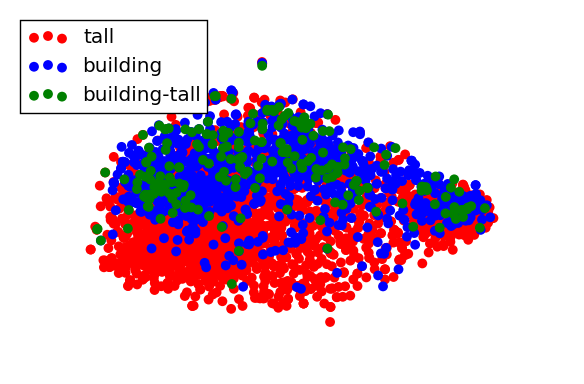
\includegraphics[width=3.5cm]{building-tall.png}}\hspace{0em}
%    \subcaptionbox{Joint}{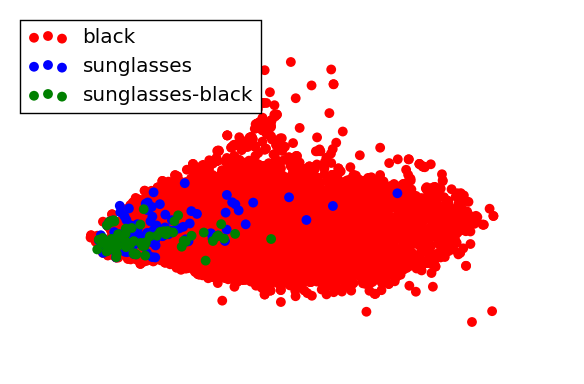
\includegraphics[width=3.5cm]{sunglasses-black.png}}\hspace{0em}
%    \subcaptionbox{Joint}{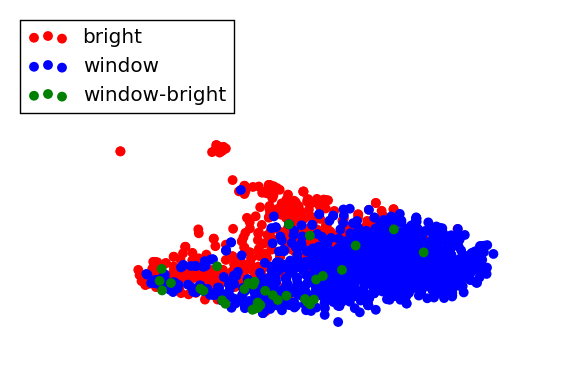
\includegraphics[width=3.5cm]{window-bright.png}}
%    \caption{Composite examples with their strategy selection: {\bf(a)} has many examples but high visual variance, {\bf(b)} is a compact visual class and {\bf(c)} has low visual variance compensating for small sample size.}%
%    \label{composites_visualizations}
%\end{figure}


\begin{table}[t]
\begin{center}
\begin{tabular}{| c || c | c | c | c | c | c | c |}
\hline
& & \multicolumn{3}{c|}{Threshold} & & &\\
Experiment & Joint & @0.25 & @0.5 & @0.75 & Independent & Multi-Att\cite{Rastegari2013} & Our Method \\ \midrule
\hline\hline
obj-att   & 0.234 & 0.238&0.243&0.247 & 0.249 & 0.234 & {\bf 0.252} \\ \midrule
\hline
obj-rel   & 0.271 & 0.270&0.270&0.269 & 0.266 & -     & {\bf 0.274} \\ \midrule
\hline
scene-att & 0.155  & 0.156&0.157&0.159 & 0.161 & 0.155 & {\bf 0.167} \\ \midrule
\hline
\end{tabular}
\end{center}
\caption{{\bf Comparison of selection strategies:} Our approach consistently outperforms all baselines in all experiments. For obj-att and obj-rel the performance is reported in Mean IoU and for scene-att in mAP.}
\label{tab:performance_summary}
\vspace*{-\baselineskip}
\vspace*{-\baselineskip}
\end{table}

\vspace{-0.05in}
\subsection{Scene classification on SUN dataset}

% \begin{figure}[t]
%     \centering
%     \subfloat{{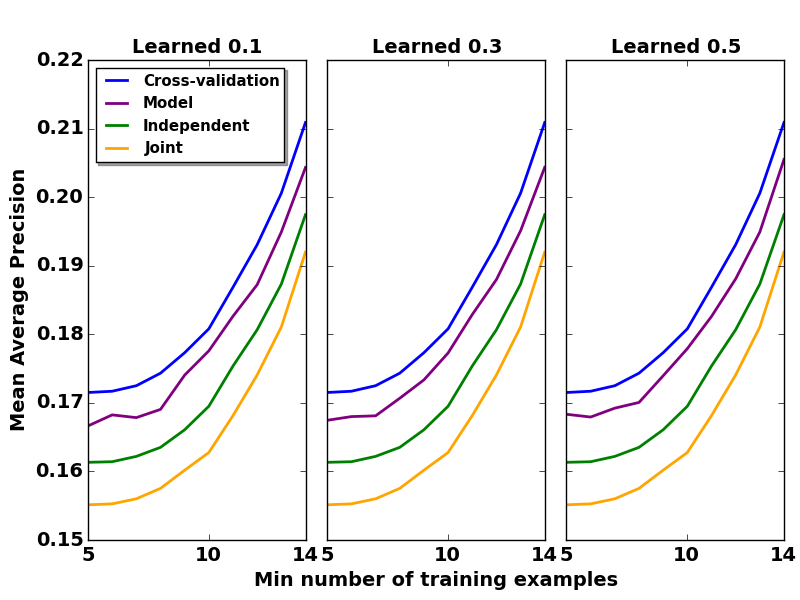
\includegraphics[width=5cm]{att_scene_multiple_partitions.png} }}%
%    \qquad
%    \subfloat{{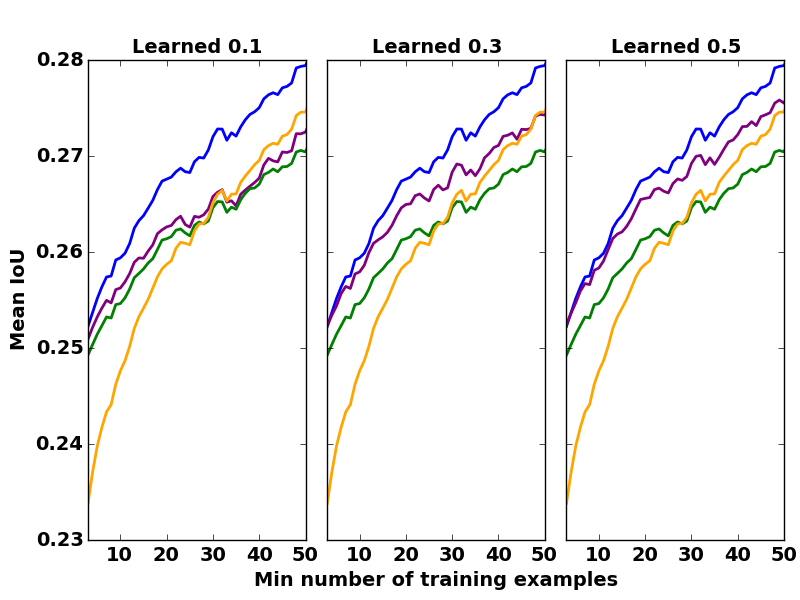
\includegraphics[width=5cm]{obj_att_multiple_partitions.png} }}%
%    \caption{Performance given different fraction of composites used for learning. Scene-attributes on SUN  (left) and object-attribute for SceneGraph dataset (right) are illustrated. Our model approaches cross-validation performance with only a fraction (0.1) of scene-attribute and (0.3) object-attribute composites.}%
%    \label{fig:example}%
    % \RevComment{Fig 3 are missing axes}
%\end{figure}

Details of the dataset, task and error metric are given in Dataset section above. Here we consider $5,071$ ($|\mathcal{C}| = 5,071$) scene-attribute composites, $C = \{s,a\}$, found in the SUN Attribute dataset. 
% , using a subset of SUN dataset annotated with 102 attributes and 717 scene categories. To overcome the small sample (5-15 positive examples per composite), We augment data resulting 10 training examples from each positive sample. 
% We perform a ranking experiment, where for each composite We rank test images by their score,obtained by the corresponding composite classifier/s. we then measure mean average precision for the top 100 ranked images. 
% We extract features $F(\mathcal{D}) = [\mathbf f_{s},\mathbf f_{a},\mathbf f_{s+a}]$ for each composite.
Results of scene-attribute query retrieval are illustrated in Table~\ref{tab:performance_summary} (bottom row). A more thorough report is given in the supplemental material, where
% Figure~\ref{fig:example} (left).
we also show performance of regressors trained with $0.1$, $0.3$, and $0.5$ fraction of the composites (tested on the rest). These experiments illustrate that we can outperform baseline strategies (and nearly match cross-validation performance) with as little as 10\% training.

% Our selection method performs better than both uniform strategies, even when using as little as $0.1$ of the composites for training. We note that the independent strategy performs better on average than the joint, due to the low number of joint training examples.

\begin{figure}[t]
    \centering
    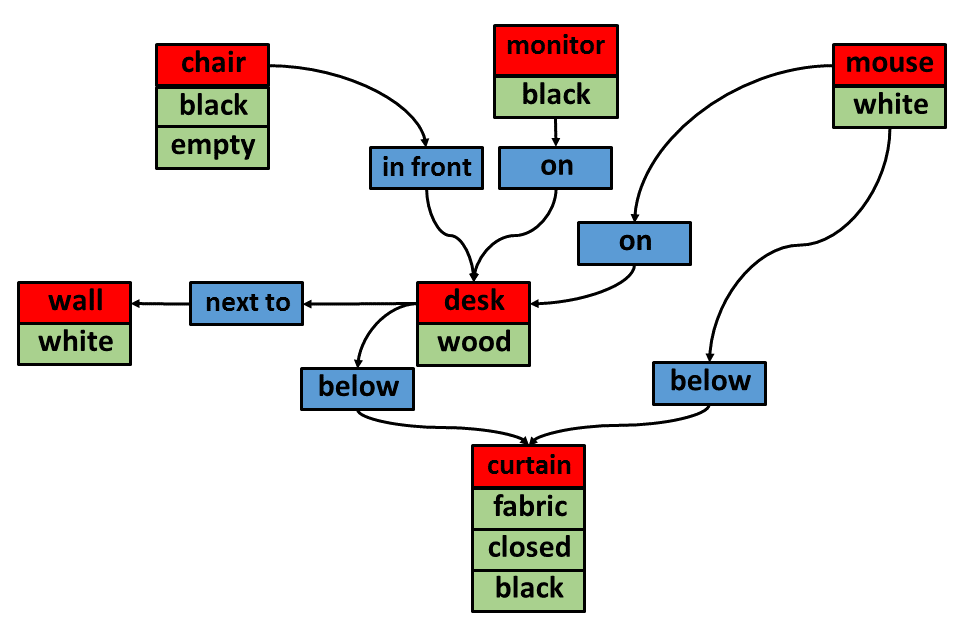
\includegraphics[width=2.7cm]{3_scene_graph.png}\hspace{0em}
    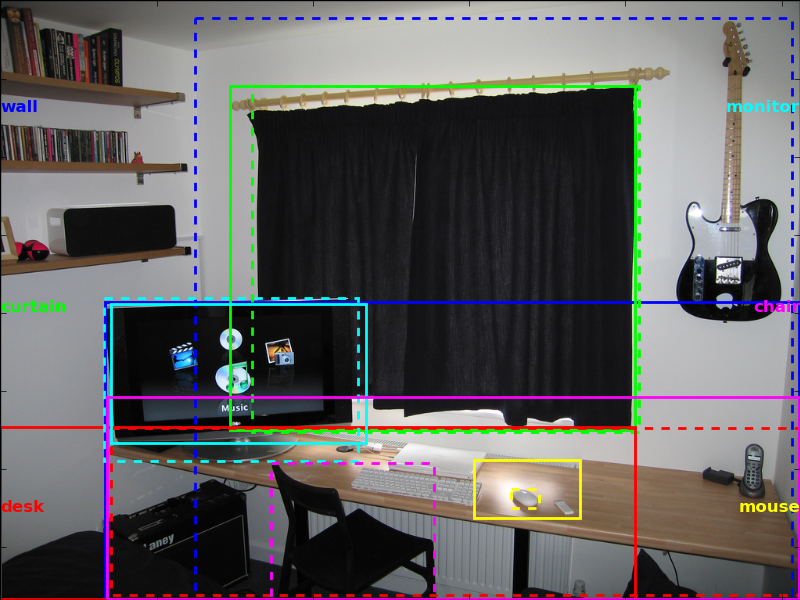
\includegraphics[width=2.7cm]{3_ind.png}\hspace{0em}
    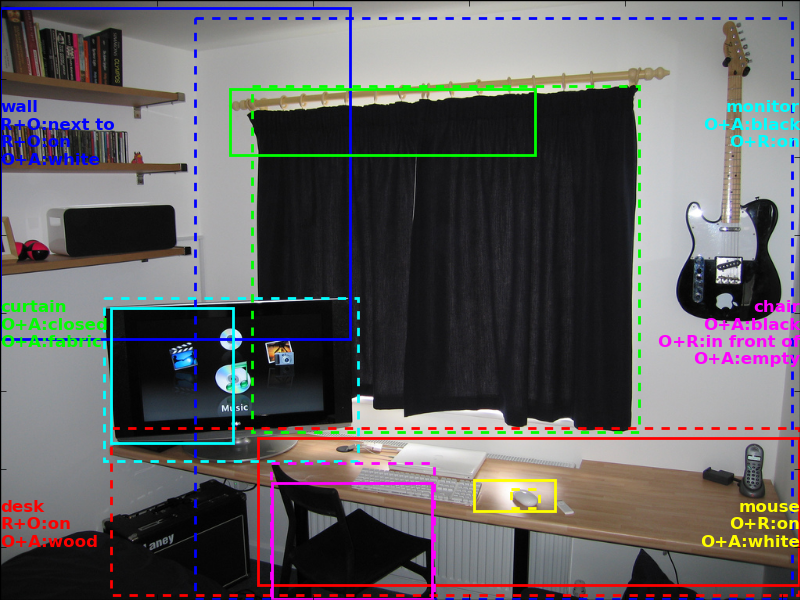
\includegraphics[width=2.7cm]{3_joint.png}\hspace{0em} 
    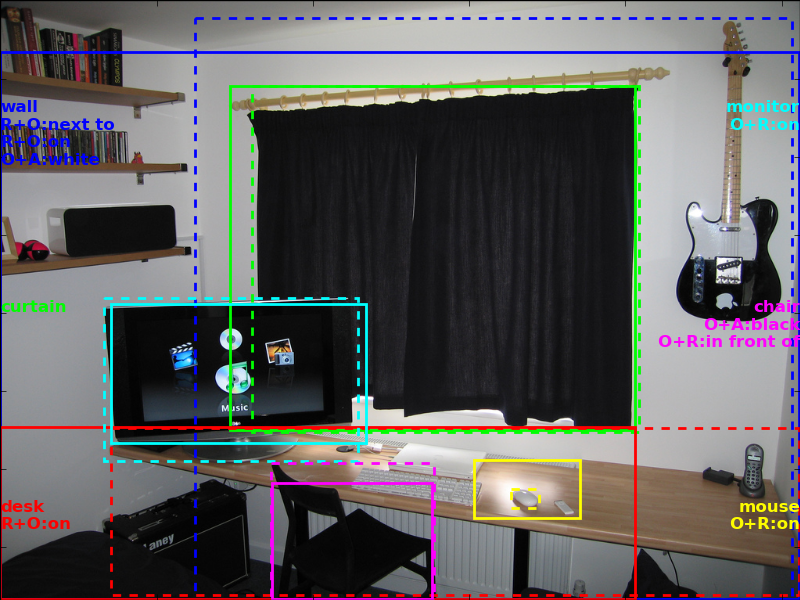
\includegraphics[width=2.7cm]{3_opt.png}
%    \vspace{0.0in}
%    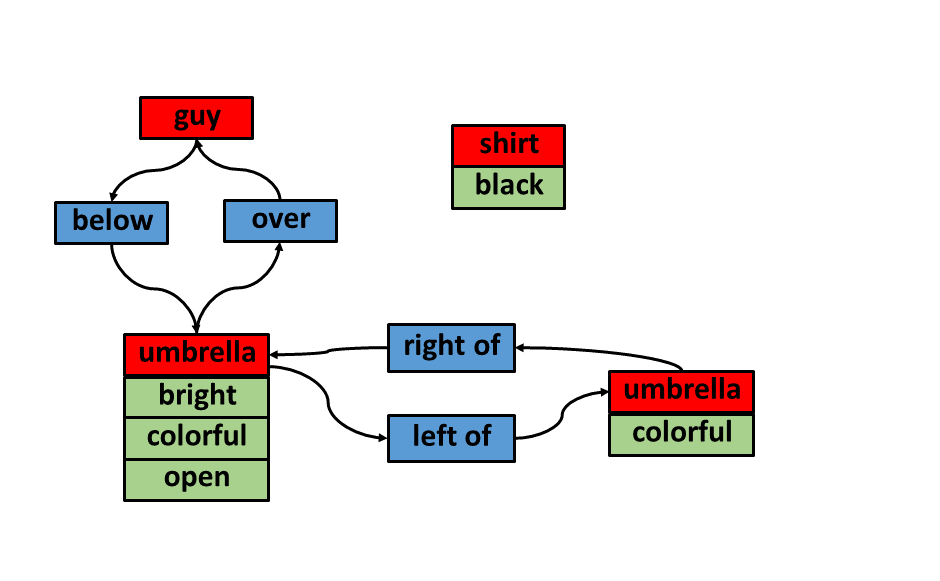
\includegraphics[width=2.7cm]{19_scene_graph.png}\hspace{0em}
%    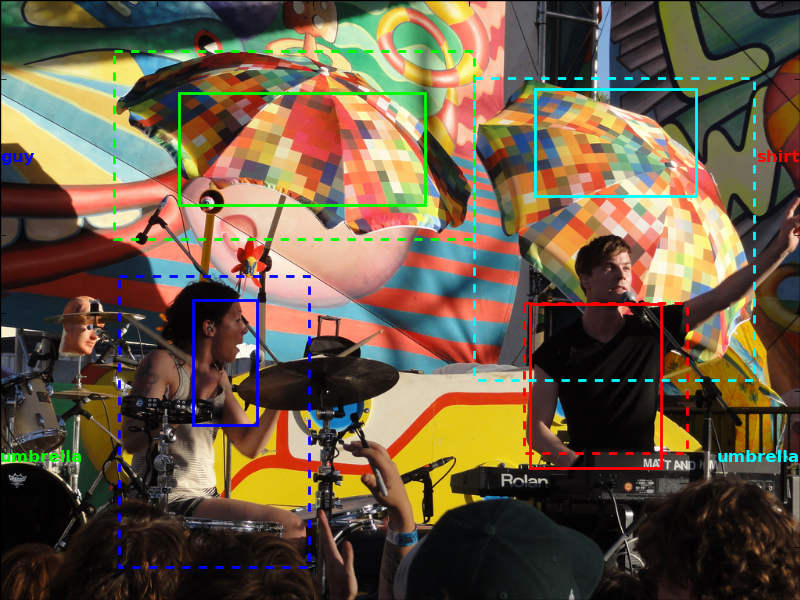
\includegraphics[width=2.7cm]{19_ind.png}\hspace{0em}
%    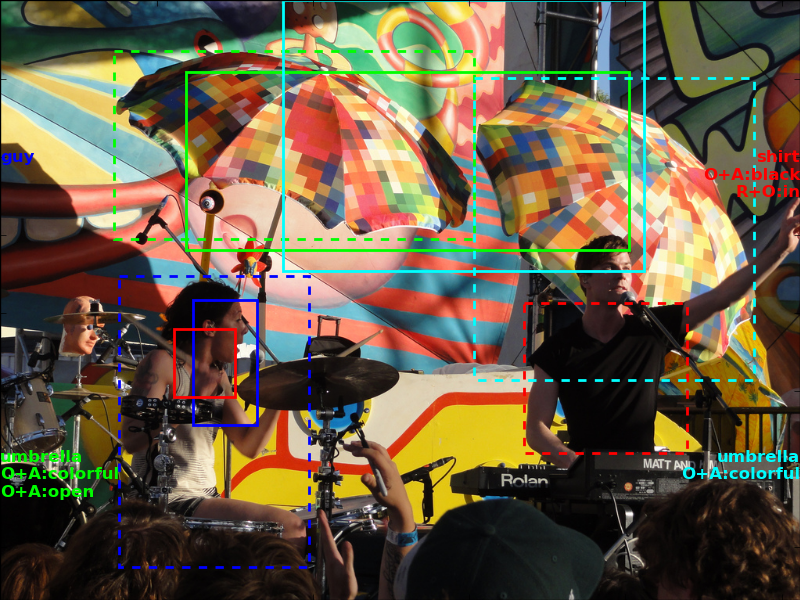
\includegraphics[width=2.7cm]{19_joint.png}\hspace{0em} 
%    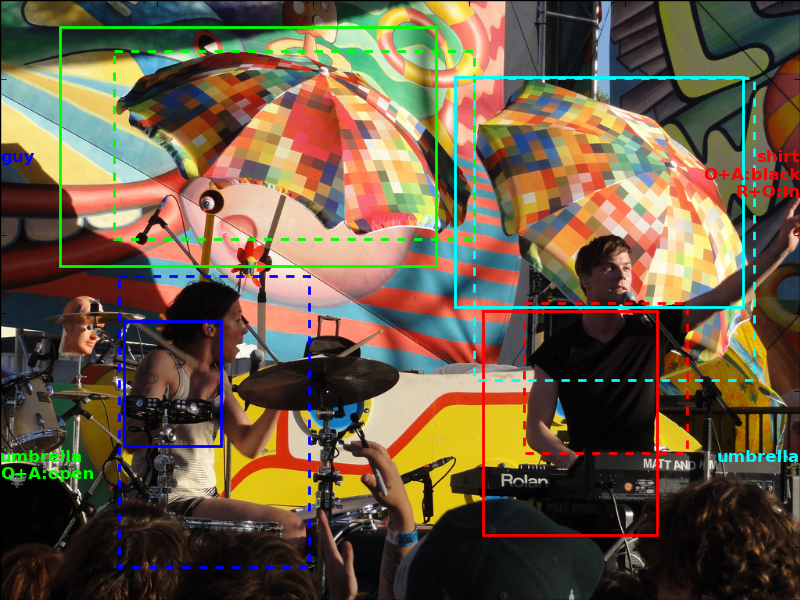
\includegraphics[width=2.7cm]{19_opt.png}
%    \vspace{0.0in}
    \centering
    \subcaptionbox{Scene graph}{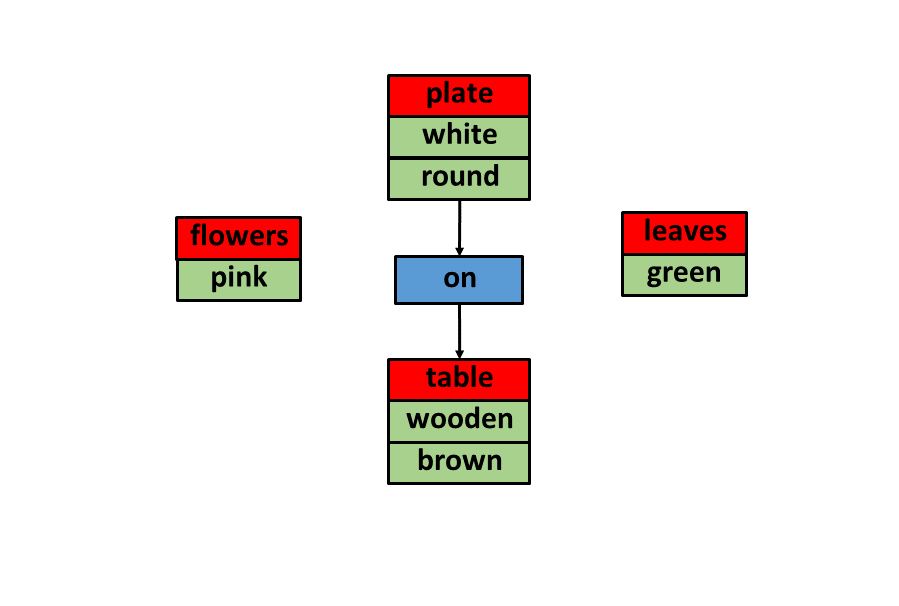
\includegraphics[width=2.7cm]{27_scene_graph.png}}\hspace{0em}
    \subcaptionbox{Independent}{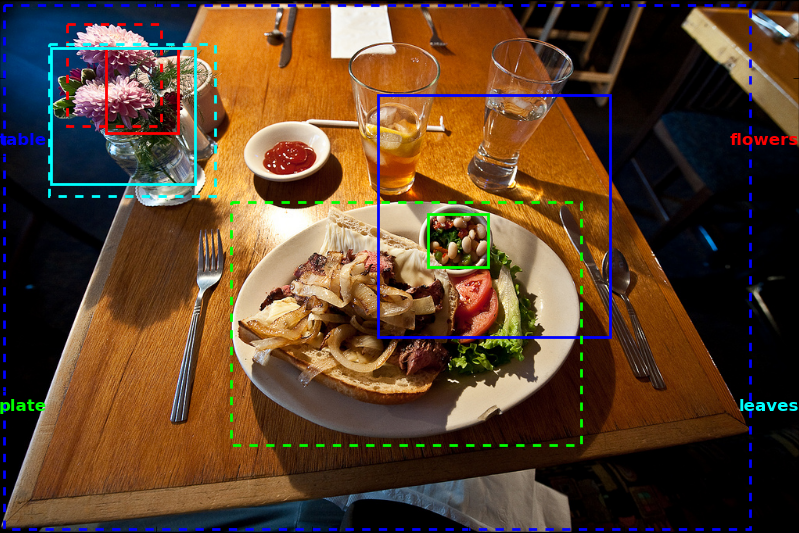
\includegraphics[width=2.7cm]{27_ind.png}}\hspace{0em}
    \subcaptionbox{Joint}{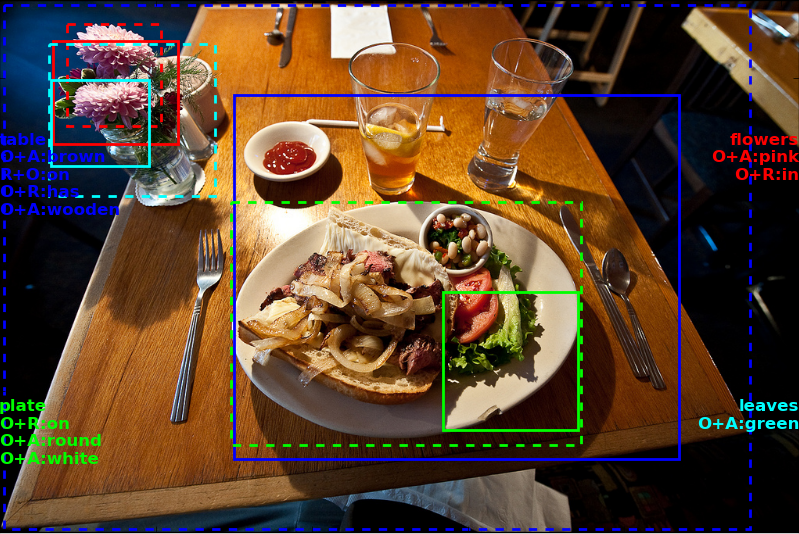
\includegraphics[width=2.7cm]{27_joint.png}}\hspace{0em} 
    \subcaptionbox{Our method}{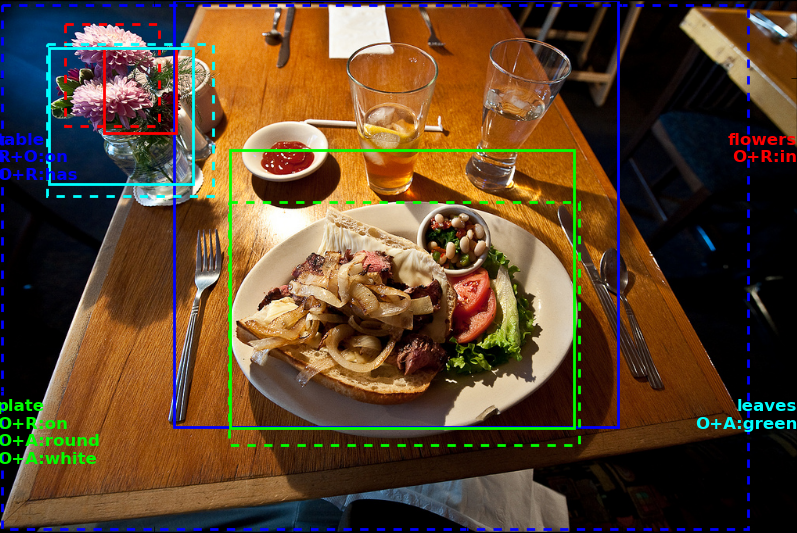
\includegraphics[width=2.7cm]{27_opt.png}}
%    \vspace{0.0in}
%    \centering
%    \subcaptionbox{Scene graph}{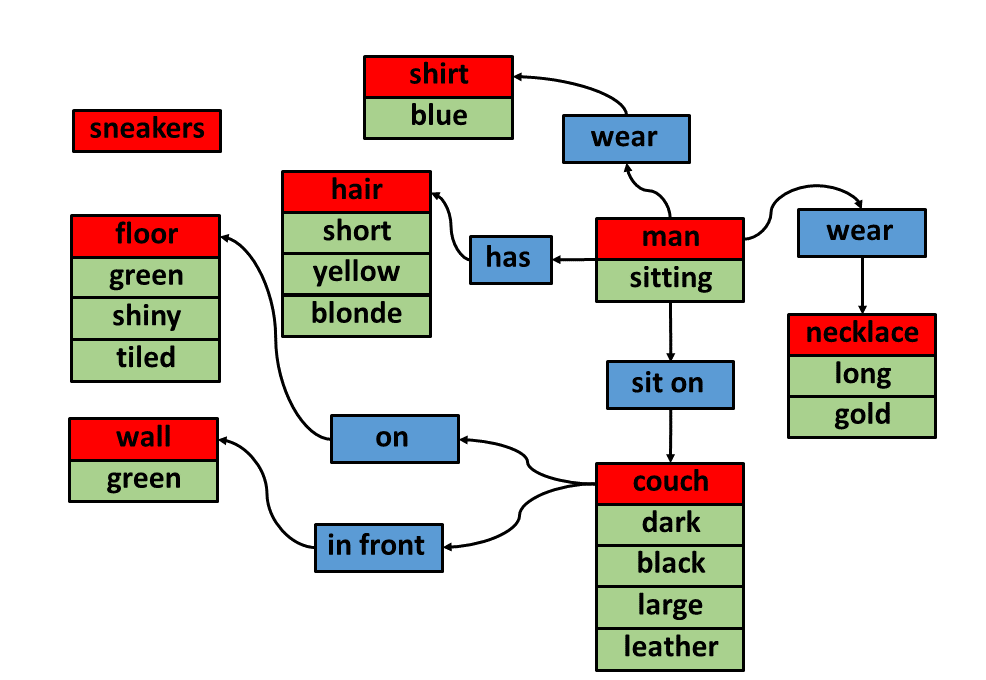
\includegraphics[width=2.7cm]{52_scene_graph.png}}\hspace{0em}
%    \subcaptionbox{Independent}{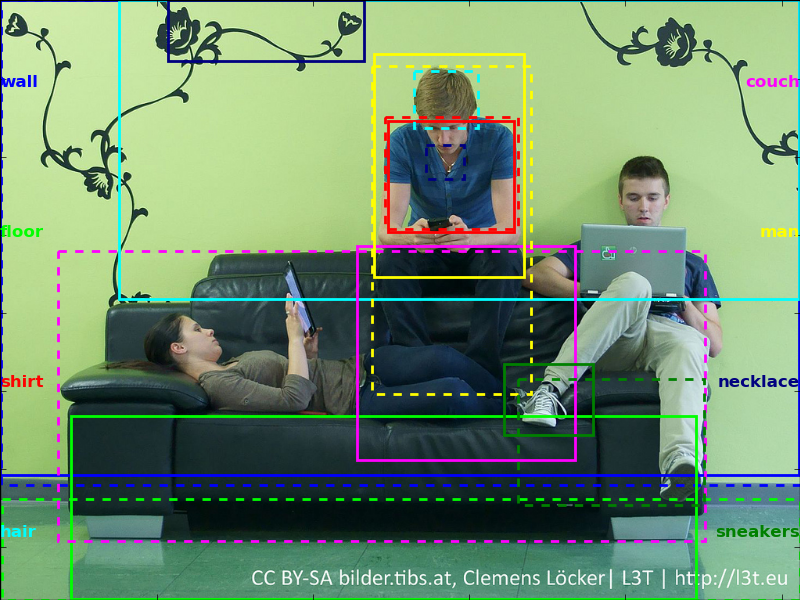
\includegraphics[width=2.7cm]{52_ind.png}}\hspace{0em}
%    \subcaptionbox{Joint}{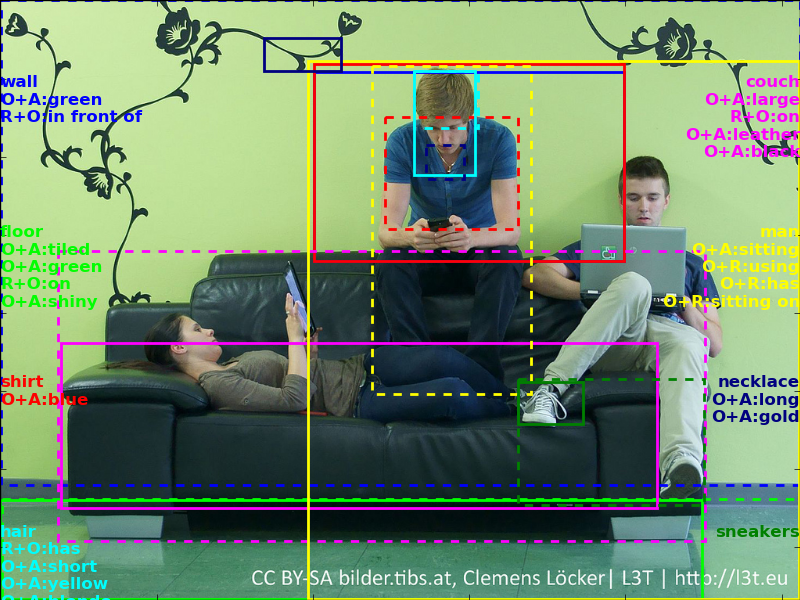
\includegraphics[width=2.7cm]{52_joint.png}}\hspace{0em}
%    \subcaptionbox{Our method}{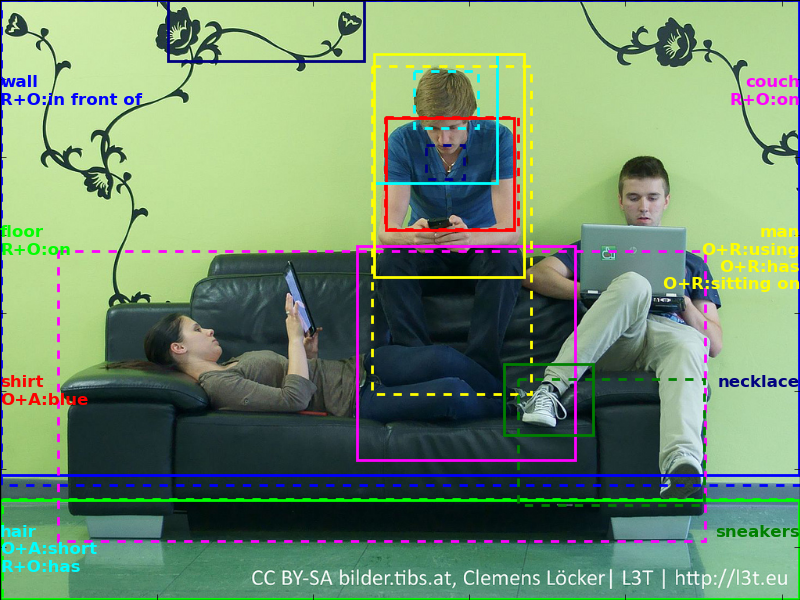
\includegraphics[width=2.7cm]{52_opt.png}}

    \caption{{\bf Qualitative results for SceneGraph retrieval:} Illustrated is (a) partial query scene graph, and grounding of objects obtained using (b) independent, (c) joint and (d) predicted, using our regression method, detector strategy. Dashed boxes are ground truth annotations.}%
    \label{scene_graph_retrieval}%
\vspace*{-\baselineskip}
% \vspace{-0.1in}    
\end{figure}

\vspace{0.07in}
\noindent
{\bf Learned Selection Strategy Evaluation:}
To further illustrate benefits of our selection strategy and compare to additional baselines, we illustrate performance across both datasets and all tasks in Table~\ref{tab:performance_summary}.
As can be seen, our method consistently outperforms uniform independent and joint selection, threshold based selection, and multi-attribute selection approach of \cite{Rastegari2013}. It should be noted that our performance, although achieves small absolute gains, is very close to cross-validation result (which is effectively our upper bound) across different datasets and experiments. We also look at and discuss the learned weights in Suppl. Mat. 
% We claim that bigger datasets (in terms of both composite number and training samples) would only improve our gain, as we expect less noisy cross-validation results. \Guy{Not sure we should say that,although it makes sense to me}. \Leon{I wouldn't. I think its implicit.}

% We also observe trends in learned weights for different experiments and datasets, as is shown in Figure~\ref{fig:learned_weights}. For example, large median pairwise distance ($\mathbf{f_4}$) of different composite parts tends to lead to joint selection, whereas large mean pairwise distance ($\mathbf{f_5}$) has the opposite effect. Some intuition for this trend is given in the right most plot.


% \RevComment{An experiment using a trivial selection criterion would be helpful. For example, using independent detectors when the number of data points is below a threshold}

\vspace{-0.05in}
\subsection{Computational efficiency}
% One can realize that our method is most useful when the training cost (in terms of both computation and time) is high. 
Because our feature space is low dimensional, is easy to compute, and the training sample, in terms of available composites, is small (order of thousands), our method has a negligible cost for training and selection prediction. In other words, when requiring $p \in (0,1)$ of the composite validation evaluations to train our method, it can save $1-p$ of the training cost. For example, it took us $5$ minutes on average to cross-validate performance of a single composite detector, using $50$ rounds of hard negative mining with $3$-fold cross validation, and less than $2$ seconds to extract features from a single composite and do prediction. 
% Our experiments show that we can match cross-validation performance when requiring 30\% pre-trained composites, hence saving at lest 70\% training cost.


% \begin{figure}
%     \centering
%     \subfloat{{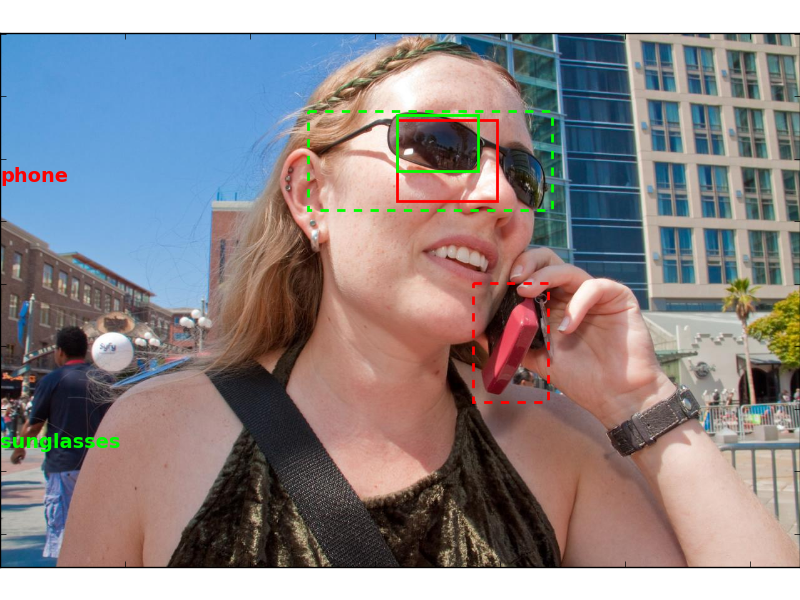
\includegraphics[width=5cm]{213_ind.png} }}%
%     \qquad
%    \subfloat{{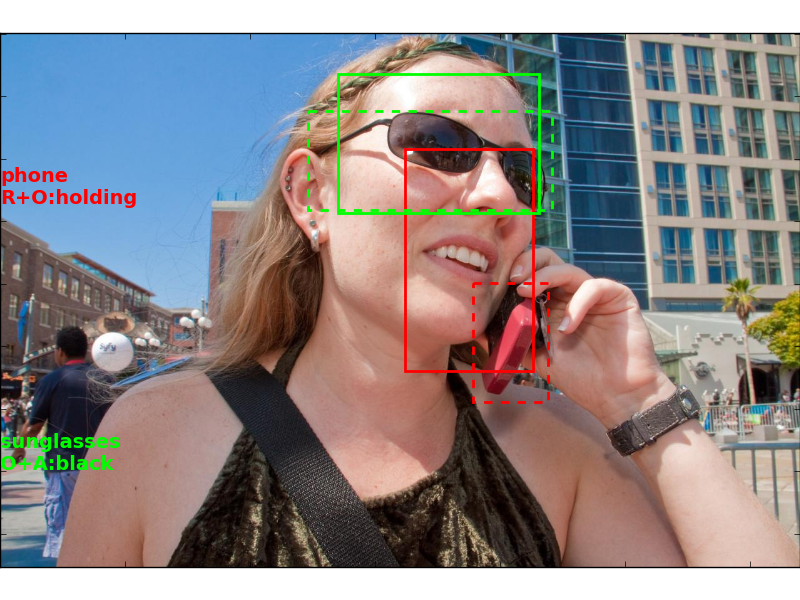
\includegraphics[width=5cm]{213_opt.png} }}%
%    \caption{Improving bad detections by using joint detectors Left: independent. Right: joint. dashed lines are ground truth}%
%    \label{fig:example}%
%\end{figure}


%-------------------------------------------------------------------------
\vspace{-0.2cm}
\section{Conclusion}

In this paper, we observed that a non-uniform selection of training strategy for visual composites can be highly beneficial. We showed that a proxy function can be learned with a small amount of data using a simple regression model, achieving similar results to cross-validation based performance. Using our model has a significant computational effect as well, offering a good speed-quality trade-off that can be utilized in various settings.



\bibliographystyle{splncs}

\bibliography{egbib}
\end{document}
